\documentclass[a4paper,14pt]{extarticle}
\usepackage{cmap}				% To be able to copy-paste russian text from pdf			
\usepackage[utf8]{inputenc}
\usepackage[T1]{fontenc}
\usepackage[margin=1in]{geometry}
\usepackage[english, russian]{babel}

\usepackage[hyphens]{url}
\urlstyle{same}
\usepackage{hyperref}

\usepackage{multirow}
\usepackage{graphicx}
\usepackage{caption}
\usepackage{amsmath}
\usepackage{mathtools}

\usepackage{tikz}
\usepackage{pgfplots}
\usepgfplotslibrary{groupplots,colorbrewer,dateplot,statistics}

%\def\ishtml{1}
\ifdefined\ishtml
  % HTML mode
  \newcommand{\urlnote}[2]{\href{#2}{#1}} % Make cool link 
  \newcommand{\smallsep}{thinspace} % to be replaced with unicode 8239 later
\else
  % PDF mode
   \usepackage{libertine}
   \usepackage{libertinust1math}
   \newcommand{\urlnote}[2]{#1\endnote{\url{#2}}}  % Put URLs to endnotes
   \newcommand{\smallsep}{\kern 0.1em}
\fi

% Move footnotes to end of document
\usepackage[backref=true]{enotez}
\DeclareTranslation{russian}{enotez-title}{Примечания}

\usepackage[
	output-decimal-marker={,},
	group-separator={\smallsep},
	group-minimum-digits=3
]{siunitx}

% Shoot me if I know a better way to make decimal groups of two
\newcommand{\rateone}[1]{\num{#1}}
\newcommand{\ratetwo}[2]{\num{#1}\smallsep#2}
\newcommand{\ratethree}[3]{\num{#1}\smallsep#2\smallsep#3}

\newcommand{\ru}[1]{\begin{otherlanguage}{russian}#1\end{otherlanguage}}
\newcommand{\en}[1]{\begin{otherlanguage}{english}#1\end{otherlanguage}}
\newcommand{\ruen}[2]{#1 (\en{#2})}

\usepackage[style=alphabetic, backend=biber]{biblatex}
\addbibresource{index.bib}
\renewcommand*{\bibfont}{\small}
\setcounter{biburllcpenalty}{9000}
\setcounter{biburlucpenalty}{9500}

\author{Артём Бакулин}
\date{\today}
\title{Индексное инвестирование}

\begin{document}

\maketitle
\thispagestyle{empty}

\begin{figure}[h]
\centering
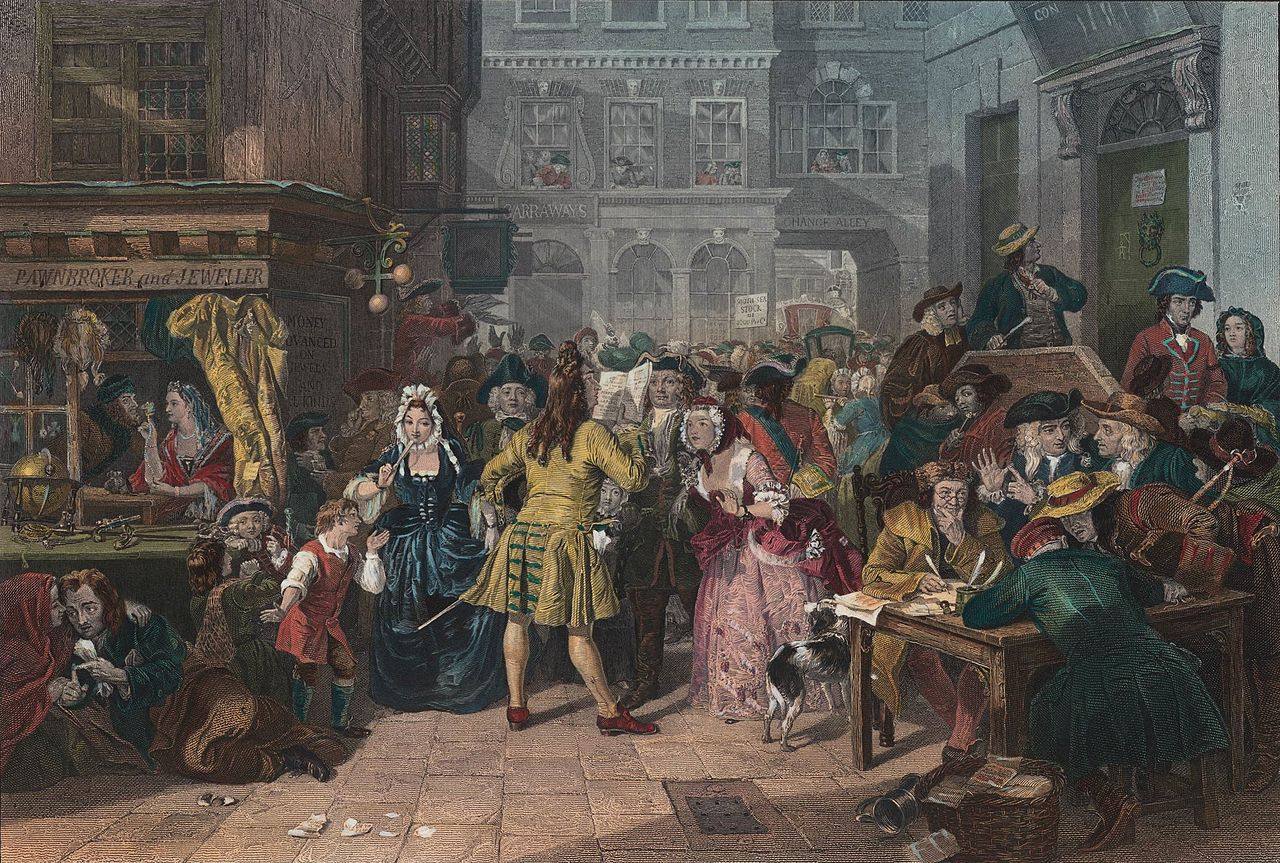
\includegraphics[width=\textwidth]{south_sea_bubble.jpg}
\captionsetup{labelformat=empty}
\caption{\small{
Эдвард Мэтью Ворд. \urlnote{Пузырь Компании Южных морей}
{https://commons.wikimedia.org/wiki/File:South_Sea_Bubble.jpg}.
1847 г. Галерея Тейт, Лондон.
}}
\end{figure}
\setcounter{figure}{0}
\newpage

\tableofcontents

\section{Рациональные инвесторы и избегание риска}

Первым делом давайте договоримся о некоторых свойствах инвесторов, которые
населяют наш уютный теоретический мирок. Как и большинство инвесторов в реальном
мире, наши сферические инвесторы будут любить доходность и не любить ненужный
риск. Из двух инвестиций с одинаковой доходностью они выберут ту, что несёт
меньший риск. Из двух инвестиций с одинаковым риском они выберут ту, что обещает
более высокую доходность.

Кому-то может показаться, что \ruen{избегание риска}{risk aversion} --- это
нерациональное поведение слабых духом homo sapiens. На деле же рациональный до
мозга костей homo economicus тоже будет избегать ненужного риска, если мы
сделаем несколько предположений о том, как он принимает решения
\cite[ch.~6.1]{bodie2014investments}.
 
Предположим, что рациональный инвестор максимизирует \ruen{функцию полезности}
{utility function}. Это означает, что все-все-все альтернативы, которые он рассматривает, подаются на вход некоторой функции $u(x)$, которая присваивает
каждой альтернативе число --- \ruen{полезность}{utility}. Из множества доступных 
альтернатив рациональный индивид всегда выбирает ту, которая даёт наибольшую
ожидаемую полезность.
 
Допустим, что функция полезности рационального инвестора --- десятичный логарифм
количества долларов на счету. Каждый новый доллар на счету увеличивает
полезность (уровень счастья), потому что логарифм --- возрастающая функция.
Кроме того, каждый следующий добавочный доллар приносит меньше счастья, чем
предыдущий, потому что логарифм --- выпуклая вверх (concave) функция. Никакие
другие параметры помимо суммы на счету нашего инвестора не интересуют.
 
Такое поведение функции полезности неплохо описывает реальное поведение людей. Согласитесь, что пятый подряд шоколадный пончик с шоколадной начинкой и шоколадной крошкой приносит меньше удовольствия, чем первый. Точно так же я на собственном опыте знаю, что десятый миллиард приносит меньше радости, чем первый.
 
Итак, рассмотрим инвестора с логарифмической полезностью. Сейчас у него на счету \$100\,000, которые дают ему $\lg 100\,000 = 5.0$ условных единиц счастья.
 
Посмотрите на такблицу \ref{logarithmic_utility_table}. Инвестор должен вложить всё своё состояние в один из двух инструментов: либо в абсолютно надёжные облигации, либо в рискованные акции. Что бы ни произошло в будущем, облигации совершенно точно вырастут на \$5\,000, и инвестор через год будет иметь \$105\,000. Акции с вероятностью 50\% вырастут на \$25\,000 и будут стоить \$125\,000, либо с вероятностью 50\% упадут на \$15\,000 и будут стоить \$85\,000. Математическое ожидание вложения в акции равно $0.5 \cdot \$85\,000 + 0.5 \cdot \$125\,000 = \$105\,000$, то есть совпадает с тем, что обещают безрисковые облигации.

\begin{table}[h!]
\centering
\begin{tabular}{l|r|r|r|r|r}
\multirow{2}{*}{Сценарий} & Вероят- & \multicolumn{2}{c|}{Облигации} & \multicolumn{2}{c}{Акции} \\
\cline{3-6}
        &  ность   & Капитал    & Полезность & Капитал      & Полезность \\ \hline
Хороший & 50\% & \$105\,000 & 5.021 & \$125\,000 & 5.097 \\
Плохой  & 50\% & \$105\,000 & 5.021 & \$85\,000  & 4.929 \\ \hline
\multicolumn{2}{l|}{Мат. ожидание}  & \$105\,000 & 5.021 & \$105\,000 & 5.013
\end{tabular}
    \caption{
        Капитал и полезность инвестора в случае инвестиций в облигации или в
        акции.
    }
    \label{logarithmic_utility_table}
\end{table}

Давайте теперь посчитаем полезность. В результате вложения в облигации инвестор получит полезность $\lg 105\,000 = 5.021$ условных единиц счастья. Если он вложится в акции, то с вероятностью 50\% акции вырастут, и полезность составит $\lg \$125\,000 = 5.097$. Однако, с вероятностью 50\% акции упадут, и полезность будет равна  $\lg 85\,000 = 4.929$. Средняя ожидаемая полезность от инвестиции в акции, таким образом, равна $0.5 \cdot 5.097 + 0.5 \cdot 4.929 = 5.013$.
 
 
Так какую же из двух альтернатив выберет наш рациональный инвестор: облигации с ожидаемой полезностью 5.021 или акции с ожидаемой полезностью 5.013? Ответ очевиден: 5.021 больше, чем 5.013, поэтому инвестор выберет облигации.

Другими словами, при одинаковой ожидаемой доходности (в обоих случаях ожидаемый капитал составляет \$105\,000) рациональный инвестор выберет менее рискованную альтернативу, то есть проявит то же самое избегание риска, что и реальные биологические инвесторы.

Как изменить условие задачи, чтобы инвестор хотя бы воспринимал две альтернативы безразлично? Можно, например, пообещать ему более высокую доходность акций в хорошем случае. Если акции будут приносить не \$125\,000, а \$129\,706, то, как показано в таблице \ref{logarithmic_utility_table_premium}, ожидаемые полезности двух альтернатив совпадут.

 \begin{table}[h!]
 \centering
 \begin{tabular}{l|r|r|r|r|r}
\multirow{2}{*}{Сценарий} & Вероят- & \multicolumn{2}{c|}{Облигации} & \multicolumn{2}{c}{Акции} \\
\cline{3-6}
        &  ность   & Капитал    & Полезность & Капитал      & Полезность \\ \hline
Хороший & 50\% & \$105\,000 & 5.021    & \$129\,706 & 5.113 \\
Плохой  & 50\% & \$105\,000 & 5.021    & \$85\,000  & 4.929 \\ \hline
\multicolumn{2}{l|}{Мат. ожидание}      & \$105\,000 & 5.021 & \$107\,353 & 5.021
\end{tabular}
\caption{Капитал и полезность инвестора в случае инвестиций в облигации или в акции. Акции имеют более высокую доходность по сравнению с таблицей \ref{logarithmic_utility_table}.}
\label{logarithmic_utility_table_premium}
 \end{table}
 
 Обратите внимание, что для того чтобы уравнять ожидаемы полезности, нам пришлось улучшить математическое ожидание дохода от акций. Раньше акции давали в среднем \$105\,000, а теперь \$107\,353, на \$2\,353 больше. Эти \$2\,353 дополнительной ожидаемой доходности --- премия за риск (risk premium), которую требует инвестор, чтобы рассмотреть возможность покупки акций. Другими словами, премия за риск уравнивает прибавку полезности в хорошем случае и снижение полезности в плохом случае. 
 
 Эти рассуждения верны не только для инвесторов с логарифмической полезностью. Достаточно, чтобы функция полезности была возрастающей и выпуклой вверх. Тогда инвесторы будут избегать риска и требовать премию (добавочную доходность) от рискованных инвестиций. Запомним эту мысль. Она пригодится, когда мы будем говорить об оптимизации портфеля и компромиссе между риском и доходностью (risk-return tradeoff).

\section{Корреляция с рынком}

Рассмотрим ещё один модельный пример. Есть две акции, каждая из которых может принести в будущем либо \$1\,000, либо \$500 с вероятностью 50/50. Акции устроены так, что когда первая приносит \$1\,000, вторая приносит \$500, и наоборот, когда первая приносит \$500, вторая приносит \$1\,000. Математическое ожидание дохода от каждой акции равно \$750. При прочих равных, какой акцией вы хотели бы владеть? Забудем о цене и предположим, что акцию вы получите в подарок.

На первый взгляд, акции совершенно симметричны. Нет никаких рациональных аргументов, чтобы предпочесть одну акцию другой. Вы могли бы подбросить монетку и положиться на случай и не прогадать. Верно? Не совсем. Что если я уточню, в каких именно сценариях акция 1 приносит \$1\,000, а в каких \$500?

Предположим, что в будущем возможны два сценария. С вероятностью 50\% вы потеряете работу (или другой источник постоянного дохода), и в этом же сценарии акция 1 будет стоить \$1\,000, а акция 2 будет стоить \$500. С вероятностью 50\% вы не только не потеряете работу, а даже получите премию \$10\,000, и в этом же сценарии акция 1 будет стоить \$500, а акция 2 будет стоить \$1\,000. Эти альтернативы перечислены в таблице \ref{two_shares_states_of_nature}.

\begin{table}[h!]
\centering
\begin{tabular}{l|r|r|r}
Сценарий                 & Вероятность & Акция 1 & Акция 2 \\  \hline
Потеря работы      & 50\%                 & \$1\,000 & \$500 \\
Премия \$10\,000 & 50\%                 & \$500      & \$1\,000 \\ \hline
\multicolumn{2}{l|}{Мат. ожидание} & \$750 & \$750 
\end{tabular}
\caption{Две акции дают одинаковую ожидаемую доходность, но приносят большую пользу в разных состояниях мира.}
\label{two_shares_states_of_nature}
\end{table}

Когда на лекции я провожу голосование среди студентов (живых людей, а не рациональных роботов), все в один голос заявляют, что предпочли бы владеть акцией 1. Это соответствует простой житейской мудрости. Акция 1 принесёт дополнительные деньги именно в <<плохом>> сценарии, когда каждый доллар на счету. Акция 1 похожа на страховку от потери работы, и поэтому люди её ценят.

Примечательно, что  рациональные логарифмические инвесторы из нашей теории будут вести себя точно так же. Из-за того что функция полезности выпукла вверх, они будут больше ценить акцию 1. Акция 1 приносит больший доход в <<плохом >> сценарии, когда каждый дополнительный доллар более ценен. С другой стороны, акция 2 приносит \$1\,000 в <<хорошем>> сценарии, когда у инвестора и так прибавится \$10\,000, и добавочная полезность от \$1\,000 будет не столь велика.

Сделаем следующий шаг. Предположим, что в нашей экономике не один рациональный инвестор, а множество. Каждый из них предпочтёт ту акцию, которая защитит его от потери работы. Что если риск потери работы для одного инвестора связан (скоррелирован) с потерей работы остальными?  Это вполне разумное предположение. Согласитесь, что для большинства людей шансы потерять работу в кризис выше, чем в хорошие времена. Кризис потому и кризис, что плохо становится сразу многим компаниям, и многие люди теряют работу одновременно.

Получается, что в среднем больше инвесторов хотят владеть <<защитной>> акцией 1. Если инвесторы покупают и продают акции на свободном рынке, то спрос на акцию 1 будет выше, чем спрос на акцию 2. При прочих равных, в равновесии акция 1 будет стоить дороже, чем акция 2.

Что это означает для доходности инвестиций в акцию 1 и акцию 2? Для начала давайте договоримся о формальном определении, что такое доходность. Допустим, что вы купили актив (акцию, облигацию, квартиру) в момент времени $t$ по цене $P_t$, а в момент времени $t+1$ актив стал стоить $P_{t+1}$. Кроме того, вы получили от актива денежную выплату (дивиденд, купон, арендную плату) $D_{t+1}$. Тогда ваша полная доходность за период времени между $t$ и $t+1$ составила
\begin{equation}
R_{t+1} = \dfrac{P_{t+1} + D_{t+1}}{P_t} - 1
\label{total_return_formula}
\end{equation}

Например, если инвестор купил акцию 2 за $P_t = \$600$, реализовался <<хороший>> сценарий, и акция стала стоить $P_{t+1} = \$1\,000$ и не заплатила никаких дивидендов ($D_{t+1} = \$0$), то инвестор заработал $\$1\,000/\$600 - 1 \approx 66.7\%$.

Если считать, что будущая цена $P_{t+1}$ и будущие дивиденды $D_{t+1}$ это случайные величины, то будущая доходность $R_{t+1}$ это тоже случайная величина, и формулу (\ref{total_return_formula}) можно записать и для математических ожиданий.
\begin{equation}
\mathbb{E}(R_{t+1}) = \dfrac{\mathbb{E}(P_{t+1}) + \mathbb{E}(D_{t+1})}{P_t}
\label{total_return_formula_exp}
\end{equation}

Выглядит как урок арифметики для старшей группы детского садика, но он показывает нам важную деталь. Текущая цена $P_t$ стоит в формулах (\ref{total_return_formula}) и (\ref{total_return_formula_exp}) в знаменателе, поэтому при той же будущей цене и будущих дивидендах более низкая цена сегодня означает большую ожидаемую доходность в будущем.

Как мы выяснили, инвесторы будут предпочитать акцию 1 акции 2. Рыночная цена акции 2 будет ниже, поэтому её ожидаемая доходность будет выше. В равновесии инвесторы будут зарабатывать более высокую доходность (большую премию за риск) на акциях, которые сильнее связаны с общим состоянием экономики, то есть растут в хорошие времена и падают плохие. Поставим крестик, чтобы вернуться к этой идее позже, когда будем изучать CAPM.

\section{Вспоминаем теорию вероятностей}

Чтобы продолжать строить теорию, нам нужно воспользоваться несколькими тривиальными фактами из теории вероятностей. Вы можете смело пропустить этот раздел, если вам не составляет труда прочитать и понять следующую фразу: <<дисперсия суммы --- это сумма дисперсий плюс две ковариации>>.

Я предполагаю, что все более-менее интуитивное понимают, что такое математическое ожидание случайной величины. Для наших целей совершенно нет необходимости знать, что это интеграл Лебега. Достаточно простой интуиции, что мат. ожидание --- это среднее значение случайной величины. Например, если мы бросаем игральный кубик, то выпавшее количество очков --- это случайная величина, которая имеет мат. ожидание $(1+2+...+6)/6=3.5$. Я буду обозначать мат. ожидание случайной величины $X$ как $\mathbb{E}(X)$.

Важное свойство мат. ожидания --- линейность. Например, если я бросаю не один кубик, а четыре, и складываю выпавшие очки, то мат. ожидание суммы будет равно $4 \cdot 3.5 =  14$. Формально это можно записать так ($\alpha$ и $\beta$ --- константы, $X$ и $Y$ --- случайные величины):
\begin{equation*}
\mathbb{E}(\alpha X + \beta Y) = \alpha\mathbb{E}(X) + \beta\mathbb{E}(Y)
\end{equation*}

Дисперсия случайной величины показывает, насколько велик разброс значений вокруг среднего. Чем больше разброс (например, чем дальше друг от друга минимум и максимум), тем больше дисперсия. Стандартное отклонение --- это квадратный корень из дисперсии. Я буду обозначать дисперсию случайной величины $X$ как  $Var(X)$, а её стандартное отклонение как $\sigma_X$.
\begin{equation*}
Var(X) = \sigma_X^2 = \mathbb{E}\left[(X - \mathbb{E}(X))^2 \right]
\end{equation*}

В примере с игральным кубиком дисперсия будет равна
\begin{equation*}
Var(X) = \dfrac{(1 - 3.5)^2 + (2 - 3.5)^2 + ... + (6 - 3.5)^2}{6} \approx 2.92
\end{equation*}

Предположим, что у нас есть две случайные величины $X$ и $Y$. Резонно задать вопрос: а есть ли связь между $X$ и $Y$? Например, верно ли, что б\'{о}льшие значения $X$ чаще выпадают одновременно с б\'{о}льшими значениями $Y$? Ответ на этот вопрос дают ковариация, которую я буду обозначать $Cov(X,Y)$, и коэффициент корреляции, который я обозначу $\rho_{X,Y}$.
\begin{equation*}
Cov(X,Y) = \rho_{X,Y}\sigma_X\sigma_Y = \mathbb{E}\left[(X - \mathbb{E}(X))(Y - \mathbb{E}(Y)) \right]
\end{equation*}

Чтобы визуализировать идею корреляции, я четыре раза попросил компьютер сгенерировать по 250 случайных реализаций стандартных нормальных величин $X$ и $Y$. Четыре эксперимента отличаются только корреляциями между $X$ и $Y$. Результаты представлены на рисунке \ref{covariance_example}. Как видите, чем ближе корреляция к 1, тем очевиднее линейная связь между $X$ и $Y$.

\begin{figure}[h!]
\centering
\begin{tikzpicture}
\begin{groupplot}[
    width = \textwidth / 3.5,
    height = \textwidth / 3.5,
    group style = {group size = 4 by 1},
    xmin = -4, xmax=4,
    ymin = -4, ymax=4
]

\nextgroupplot[title = {$\rho_{X,Y}=0.0$}]
\addplot[color=Set1-B, only marks] table[x=X0, y=Y0, col sep=comma] {data/covariance_plot_random_samples.csv};

\nextgroupplot[title = {$\rho_{X,Y}=0.25$}]
\addplot[color=Set1-B, only marks] table[x=X25, y=Y25, col sep=comma] {data/covariance_plot_random_samples.csv};

\nextgroupplot[title = {$\rho_{X,Y}=0.75$}]
\addplot[color=Set1-B, only marks] table[x=X75, y=Y75, col sep=comma] {data/covariance_plot_random_samples.csv};

\nextgroupplot[title = {$\rho_{X,Y}=1.0$}]
\addplot[color=Set1-B, only marks] table[x=X100, y=Y100, col sep=comma] {data/covariance_plot_random_samples.csv};

\end{groupplot}
\end{tikzpicture}
\caption{Реализации случайных величин $X$ и $Y$ в зависимости от корреляции между ними.}
\label{covariance_example}
\end{figure}

Нам понадобится правило для вычисления дисперсии суммы случайных величин. Дисперсия суммы зависит как от дисперсии слагаемых, так и от ковариации (или от корреляции) между ними:
\begin{align}
Var(\alpha X + \beta Y) &= \alpha^2 Var(X) + \beta^2 Var(Y) + 2 \alpha \beta Cov(X, Y) = \nonumber \\
&= \alpha^2\sigma_X^2 + \beta^2 \sigma_Y^2 + 2\alpha\beta\rho_{X,Y}\sigma_X\sigma_Y
\label{variance_of_linear_combination}
\end{align}

\section{Диверисификация, или о пользе корреляций}

Если бы я мог дать вам всего один совет касательно инвестиций, то я бы сказал <<диверсифицируйтесь!>>. Или, следуя народной мудрости, не кладите все яйца в одну корзину. 

Есть несколько довольно популярных заблуждений по поводу диверсификации. Первое --- что диверсификация уменьшает доходность. Второе --- что диверсификация возможна, только если активы, в которые вы инвестируете, связаны отрицательной корреляцией. Это не так, и если вы, как и остальные инвесторы, не любите риск и любите доходность, то вы можете улучшить баланс риска и доходности с помощью диверсификации.

Рассмотрим пример. Пусть у нас есть всего две акции, $X$ и $Y$. Мы знаем, что они имеют одинаковую ожидаемую доходность $\mu=5\%$ и одинаковое стандартное отклонение $\sigma=10\%$. Кроме того, они связаны друг с другом корреляцией  $\rho_{X,Y} = 0.4$. Вы должны вложить долю $w$ своего капитала в акции $X$, а долю $(1-w)$ --- в акции $Y$.

Зависит ли ожидаемая доходность ваших инвестиций от выбора $w$? Нет, не зависит. Из линейности мат. ожидания следует, что при любом выборе $w$ вы всегда получите одну и ту же ожидаемую доходность 5\%:
\begin{equation*}
\mathbb{E}\left[ wX + (1-w)Y\right] = w\mathbb{E}(X) + (1-w)\mathbb{E}(Y) = w\mu + (1-w)\mu = \mu = 5\%
\end{equation*}

А что с риском? Из формулы (\ref{variance_of_linear_combination}) следует, что дисперсия и стандартное отклонение зависят не только от стандартного отклонения каждой акции, но и от корреляции между ними:
\begin{align*}
Var(wX + (1-w)Y)
&= w^2Var(X) + (1-w)^2Var(Y) + 2w(1-w)Cov(X,Y) = \\
&= w^2\sigma^2 + (1-w)^2\sigma^2 + 2w(1-w)\rho_{X,Y}\sigma^2 = \\
&= \sigma^2\left(w^2 + (1-w)^2 + 2w(1-w)\rho_{X,Y} \right)
\end{align*}

Невооружённым глазом видно, что дисперсия портфеля (то есть риск) есть квадратичная функция от $w$. Стало быть, при каком-то $w$ она должна достигать минимума. Как показано на рисунке \ref{portfolio_volatility_vs_w}, этот минимум действительно достигается при $w=0.5$, то есть если вы инвестируете половину капитала в акции $X$ и половину в акции $Y$. Стандартное отклонение доходности вашего портфеля составит 8.37\%. С другой стороны, если бы вы инвестировали все деньги только в акцию $X$ (или наоборот, только в акцию $Y$), то вам бы пришлось смириться со стандартным отклонением целых 10\%.

\begin{figure}[h!]
\centering
\begin{tikzpicture}
\begin{axis}[
  width = \textwidth * 0.5,
  xlabel={$w$ --- доля инвестиций в акцию $X$},
  ylabel={Ст. откл. портфеля, \%},
  xmin=0, xmax=1,
  ymin=0, ymax=10,
  yticklabel={$\pgfmathprintnumber{\tick}$}
]
   \addplot[
        color = Set1-B,
		  line width = 1pt,
		  samples at = {0,0.05,...,1}
	]
	{10 * sqrt(x^2 + (1-x)^2 + 2*0.4*x*(1-x))};

	\draw[
		color=black,
		dashed
	]
	(axis cs: 0.5, 0) -- (axis cs: 0.5, 8.366) -- (axis cs: 0, 8.366);

	\node[
		anchor=north west
	]
	at (axis cs: 0.5, 8.366)
	{(0.5, 8.37\%)};

    \node[
        color=Set1-B,
        circle,
        fill, 
        inner sep=2pt
    ]
    at (axis cs: 0.5, 8.366) {};
\end{axis}
\end{tikzpicture}
\caption{Зависимость стандартного отклонения доходности портфеля от доли инвестиций в акцию $X$.}
\label{portfolio_volatility_vs_w}
\end{figure}

Вывод: вам не нужно искать активы с отрицательной корреляцией, чтобы воспользоваться плодами диверсификации! Вполне достаточно, чтобы корреляция была отлична от 1.0. Диверсификация может снизить риск ваших инвестиций при той же ожидаемой доходности или дать б\'{о}льшую доходность при неизменном уровне риска.

\section{Портфельная оптимизация}

Давайте обобщим наш замечательный пример с двумя акциями на случай, когда мы составляем портфель из произвольного числа активов. При этом каждый актив обладает собственной ожидаемой доходностью и дисперсией.

Допустим, что нам известны ожидаемые доходности четырёх активов: акций, облигаций, \ruen{инвестиционных фондов недвижимости}{real estate investment trust, REIT} и золота. Также мы знаем стандартные отклонения и корреляции между активами. Эти значения приведены в таблице \ref{asset_class_returns_table}.

\begin{table}[h!]
\centering
\begin{tabular}{l|r|r|r|r|r|r}
 & \multicolumn{2}{c|}{Доходность} & \multicolumn{4}{c}{Корреляция} \\ \cline{2-7}
Актив        & Среднее & Ст. откл. & Акц. & Обл. & Нед. & Зол. \\ \hline
Акции        & 10.9\%  & 15.2\%    & 1.00  & 0.00   & 0.59    & 0.04 \\
Облигации    & 5.2\%   & 3.6\%     & 0.00  & 1.00   & 0.19    & 0.28 \\
Недвижимость & 10.8\%  & 19.2\%    & 0.59  & 0.19   & 1.00    & 0.13 \\
Золото       & 7.0\%   & 15.6\%    & 0.04  & 0.28   & 0.13    & 1.00
\end{tabular}
\caption{Средние доходности, стандартные отклонения и корреляции между классами активов. Период 1994--2020 по данным сайта \urlnote{Portfolio Visualizer}{https://www.portfoliovisualizer.com/efficient-frontier}.}
\label{asset_class_returns_table}
\end{table}

Как видите, я использовал \emph{исторические} данные, чтобы оценить параметры распределения \emph{будущих} доходностей активов. Это довольно опасное занятие, потому что прошлое не предсказывает будущее. В идеале, я должен был бы нанять аналитика, который выдал бы мне ожидаемые будущие доходности исходя из научного прогноза, а не исходя из средней доходности в прошлом. К сожалению, редкий прогноз на финансовых рынках оказывается точнее, чем <<будет как раньше>>. Впрочем, для нашей цели проиллюстрировать принцип диверсификции это не так важно.

Итак, вы --- инвестор, который любит доходность и не любит дисперсию. Вам нужно распределить свой капитал между четырьмя активами. Какую пропорцию между акциями, облигациями, недвижимостью и золотом выбрать?

Разумно задать следующий вопрос: если вы хотите получить ожидаемую доходность, скажем 10\%, то какой портфель (какая пропорция акций, облигаций, недвижимости и золота) обеспечат такую доходность? А если таких возможных портфелей несколько (что вполне возможно), то который из них будет наименее рискованным (дисперсия и стандартное отклонение будут меньше, чем у остальных портфелей с такой доходностью)?

Рисунок \ref{efficient_frontier} отвечает на этот вопрос. Каждая точка на графике --- это гипотетический портфель, который характеризуется стандартным отклонением (ось $x$) и ожидаемой доходностью (ось $y$). Для каждого уровня желаемой доходности я рассчитал (как --- расскажу позже) оптимальный портфель, то есть портфель с наименьшим стандартным отклонением из всех портфелей с данной доходностью. %Например, если вас удовлетворит доходность 6.5\%, то я рекомендую вам портфель из 21.2\% акций, 74.6\% облигаций, 0.5\% недвижимости и 3.7\% золота.

\begin{figure}[h!]
\centering
\begin{tikzpicture}
\begin{axis}[
    width=\textwidth,
    xlabel={Стандартное отклонение, \%},
    ylabel={Ожидаемая доходность, \%},
    xmin=0, xmax=21,
    ymin=0, ymax=13
]

\newcommand{\drawAssetNode}[3]{
    \node[
        circle,
        fill,
        inner sep=2pt
    ] at (axis cs: #1, #2) {};
    \node[
        anchor=north
    ]
    at (axis cs: #1, #2)
    {\small #3};
}

\newcommand{\drawPortfolioNode}[8]{
    \node[
        anchor=#8
    ] at (axis cs: #1, #2) {
	     \small
	     \begin{tabular}{|l|r|}
		  \hline
		  \multicolumn{2}{|c|}{#3} \\ \hline
		  Акц. & #4\% \\
		  Обл. & #5\% \\
		  Нед. & #6\%  \\
		  Зол. & #7\% \\
		  \hline
		  \end{tabular}
    };
	 
	 \node[
	     circle,
	     fill,
	     inner sep=3pt,
	     color=Set1-B
    ] at (axis cs:#1, #2) {};
}

\addplot[
    line width=1pt,
    color=Set1-B
]
table[
    x=std_dev,
    y=target_return,
    col sep=comma
]
{data/efficient_frontier_plot_data.csv};

\drawAssetNode{15.2}{10.9}{Акции}

\drawAssetNode{3.6}{5.2}{Облигации}

\drawAssetNode{19.2}{10.8}{Недвиж.}

\drawAssetNode{15.6}{7.0}{Золото}

\drawPortfolioNode{4.40}{6.5}{Портфель 1}{21.2}{74.6}{0.5}{3.7}{south east}

\drawPortfolioNode{12.0}{9.95}{Портфель 2}{63.2}{3.5}{14.4}{18.9}{south east}

\drawPortfolioNode{12.0}{6.5}{Портфель 3}{0.0}{30.0}{0.0}{70.0}{north east}

\draw[dashed] (axis cs: 12.0, 9.95) -- (axis cs: 12.0, 0);
\draw[dashed] (axis cs: 0.0, 6.5) -- (axis cs: 12.0, 6.5);
\draw[dashed] (axis cs: 0, 9.95) -- (axis cs: 12.0, 9.95);
\draw[dashed] (axis cs: 4.40, 0) -- (axis cs: 4.40, 6.5);

\end{axis}
\end{tikzpicture}

\caption{Граница эффективности для портфелей, составленных из акций, облигаций, недвижимости и золота.}
\label{efficient_frontier}
\end{figure}

Синяя линия на графике --- это так называемая \ruen{граница эффективности}{efficient frontier}. Именно на ней лежат оптимальные портфели, имеющие минимальное стандартное отклонение при заданной доходности. Рациональный инвестор будет стремиться выбрать один из портфелей на этой линии, потому что любой другой портфель будет заведомо хуже.

Например, совершенно нет смысла выбирать портфель 3, состоящий на 30\% из облигаций и 70\% из золота. Этот портфель имеет ожидаемую доходность 6.5\% при стандартном отклонении 12\%. Однако, раз уж вы согласны принять на себя риск в 12\%, то за этот риск вы можете получить намного более высокую доходность --- почти 10\% в портфеле 2 (63.2\% в акциях). С другой стороны, если вы готовы удовлетвориться ожидаемой доходностью 6.5\%, то лучше выбрать намного менее рискованный портфель 1 (74.6\% в облигациях), который имеет стандартное отклонение 4.4\%.

Другими словами, вы всегда стремитесь выбрать портфель, который лежит выше (больше доходность) и левее (меньше риск). В какой-то момент вы упрётесь в границу эффективности и не сможете двигаться дальше --- не получится заработать 15\% при стандартном отклонении 2\%. Очутившись на границе эффективности, вы можете гулять по ней либо вправо-вверх (больше риск, больше доходность), либо влево-вниз (ниже риск, ниже доходность). То, на каком из оптимальных портфелей на границе эффективности остановитесь именно вы, зависит от вашей личной чувствительности к риску.

Обратите внимание, что граница эффективности лежит выше или левее, чем отдельные активы --- облигации, золото, недвижимость. Мы снова возвращаемся к идее диверсификации. Если вы держите все инвестиции в одном активе, то скорее всего вы могли бы получать такую же доходность при меньшем уровне риска, если бы диверсифицировались. Чаще всего на границе эффективности оказываются портфели, составленные из нескольких активов.

Рисунок \ref{efficient_frontier_allocation} показывает, как изменяется состав оптимального портфеля по мере того как вы движетесь по границе эффективности слева направо (от меньшего риска к большему риску). Вполне ожидаемо, наименее рискованные портфели состоят в основном из облигаций, а наиболее рискованные --- из акций и недвижимости.

\begin{figure}[h!]
\centering
\begin{tikzpicture}
\begin{axis}[
  width=\textwidth,
  height=\textwidth/2,
  xlabel={Стандартное отклонение, \%},
  ylabel={Доля актива, \%},
  xmin=3.5, xmax=15.2,
  ymin=0, ymax=100,
  stack plots=y
]

\node at (axis cs:9.3, 25) {\small Акции};
\node at (axis cs:9.3, 63) {\small Облигации};
\node at (axis cs:9.3, 82) {\small Недвиж.};
\node at (axis cs:9.3, 93) {\small Золото};

\addplot[fill=Pastel2-C] table[x=std_dev, y=stocks, col sep=comma] {data/efficient_frontier_plot_data.csv} \closedcycle;

\addplot[fill=Pastel2-D] table[x=std_dev, y=bonds, col sep=comma] {data/efficient_frontier_plot_data.csv} \closedcycle;

\addplot[fill=Pastel2-E] table[x=std_dev, y=reit, col sep=comma] {data/efficient_frontier_plot_data.csv} \closedcycle;

\addplot[fill=Pastel2-F] table[x=std_dev, y=gold, col sep=comma] {data/efficient_frontier_plot_data.csv} \closedcycle;
\end{axis}
\end{tikzpicture}

\caption{Состав портфелей на границе эффективности.}
\label{efficient_frontier_allocation}
\end{figure}

В подтверждение тезиса о диверсификации, единственный оптимальный портфель, который состоит только из одного актива (акций) --- это портфель с максимальной доходностью и максимальным риском. Это ожидаемо, потому что в условии задачи именно акции имеют максимальную доходность 10.9\%. Если хоть немного разбавить акции другим активом с меньшей доходностью, то общая доходность портфеля упадёт. Так что инвестор, который желает выжать максимально возможную доходность, будет вынужден составить портфель только из акций.

\section{Квадратичное программирование}

В предыдущем разделе я обещал рассказать, как именно я посчитал оптимальные портфели. В этом разделе я выполню обещание и объясню, как формально поставить задачу выбора оптимального портфеля на языке математики. Если вам не очень интересны математические подробности, то вы можете смело перейти к следующему разделу. Незнание этих выкладок не помешает вам продолжить читать статью и извлечь из неё пользу. Если же вы всё ещё со мной, то, как говорил известный сатирик, наберите воздуха в грудь.

Итак, у нас есть $n$ активов. Будущая доходность $i$-го актива --- это случайная величина со средним $\mu_i$ и стандартным отклонением $\sigma_i$. Доходности $i$-го и $j$-го актива связаны корреляцией $\rho_{i,j}$.

Нас просят распределить единичный капитал между активами. Более формально, $i$-му активу нужно присвоить вес (долю в портфеле) $x_i$. Потребуем, чтобы все веса $x_i$ были положительными (нельзя продать актив, которого у нас нет), а их сумма равнялась единице (мы должны распределить весь капитал без остатка). 

Для начала введём несколько удобных матричных обозначений, то есть запишем параметры задачи в аккуратные прямоугольные таблицы.
\begin{align*}
x = \begin{bmatrix}x_1 \\ x_2 \\ \vdots \\ x_n\end{bmatrix}
\qquad
\mu = \begin{bmatrix}\mu_1 \\ \mu_2 \\ \vdots \\ \mu_n\end{bmatrix}
\qquad
S = \begin{bmatrix}
\sigma_1^2 & \rho_{1,2}\sigma_1\sigma_2 & \cdots & \rho_{1,n}\sigma_1\sigma_n \\
\rho_{2,1}\sigma_2\sigma_1 & \sigma_2^2 & \cdots & \rho_{2,n}\sigma_2\sigma_n \\
\vdots & \vdots & \ddots & \vdots \\
\rho_{n,1}\sigma_n\sigma_1 & \rho_{n,2}\sigma_n\sigma_2 & \cdots & \sigma_n^2
\end{bmatrix}
\qquad
e = \begin{bmatrix}1 \\ 1 \\ \vdots \\ 1\end{bmatrix}
\end{align*}

Утверждается, что вопрос <<какой портфель с ожидаемой доходностью $r$ имеет наименьшую дисперсию?>> можно формально записать в виде следующей задачи минимизации:
\begin{align}
\begin{cases}
x^TSx \to \min \\
\mu^Tx = r \\
e^Tx = 1 \\
x \ge 0
\end{cases}
\label{portfolio_optimization_statement}
\end{align}

Вид формул (\ref{portfolio_optimization_statement}) вызывает у разных людей противоположные эмоции. Например, человек, знакомый с теорией математической оптимизации, воскликнет <<Батюшки, да это же банальный QP! Стоило ли ради этого писать столько текста?>>.

Действительно, хорошая новость заключается в том, что человечество уже давно научилось решать задачи такого вида и даже дало им специальное название --- \ruen{квадратичное программирование}{quadratic programming, QP} \cite[ch.~7--8]{cornuejols2006optimization}. Почти для любого языка программирования, от C до Питона, найдётся готовая библиотека для решения этой задачи. Достаточно ничего не напутать и правильно составить матрицы $\mu$, $S$ и $e$, а дальше библиотека сама найдёт оптимальное решение. Совершенно не обязательно разбираться в том, какой алгоритм поиска решения крутится под капотом .

С другой стороны, у неподготовленного человека такая постановка задачи может вызвать ступор. Давайте пройдёмся по ней строчка за строчкой, чтобы убедиться, что в ней нет никакой тёмной магии.

Что такое $x^TSx$? Это компактная запись дисперсии портфеля, составленного с весами $x_i$. Для наглядности можно расписать это выражение для случая двух активов ($n=2$) и перемножить матрицы, как нас учили на первом курсе (строка на столбец). Получится уже знакомая нам формула (\ref{variance_of_linear_combination}), связывающая дисперсию суммы с ковариацией:
\begin{align*}
x^TSx &= 
\begin{bmatrix}x_1 & x_2\end{bmatrix}
\begin{bmatrix}
\sigma_1^2 & \rho_{1,2}\sigma_1\sigma_2 \\
\rho_{1,2}\sigma_1\sigma_2 & \sigma_2^2
\end{bmatrix}
\begin{bmatrix}
x_1 \\
x_2
\end{bmatrix}
=
\begin{bmatrix}x_1 & x_2\end{bmatrix}
\begin{bmatrix}
x_1\sigma_1^2 + x_2\rho_{1,2}\sigma_1\sigma_2 \\
x_1\rho_{1,2}\sigma_1\sigma_2 + x_2\sigma_2^2
\end{bmatrix} = \\
&= 
x_1^2\sigma_1^2 + 2x_1x_2\rho_{1,2}\sigma_1\sigma_2 + x_2^2\sigma_2^2
\end{align*}

Следовательно, если мы попросим алгоритм минимизировать значение $x^TSx$, то он постарается найти портфель (набор весов $x_i$) с минимальной дисперсией.

Если не дать алгоритму оптимизации никаких ограничений, то он довольно быстро скажет вам, что портфель с минимальной дисперсией --- это портфель с нулевыми весами. Действительно, если ничего не инвестировать, то и риска никакого не будет. Однако, это не совсем то, что мы хотим, поэтому нам нужно добавить в задачу дополнительные \ruen{ограничения}{constraints}.

Первое условие --- это $\mu^Tx = r$. По-русски, мы просим алгоритм рассматривать только те портфели, которые имеют ожидаемую доходность $r$. В самом деле, если расписать матричное умножение, то получится сумма $\mu_1x_1 + ... + \mu_nx_n$, то есть ожидаемая доходность портфеля.

Второе условие --- это $e^Tx = 1$. Его можно записать как $x_1 + ... + x_n = 1$. Мы говорим алгоритму, что корректное решение (набор весов $x_i$) --- это когда весь единичный капитал распределён между активами и ни один рубль не остался неинвестированным.

Наконец, третье условие $x \ge 0$ просто говорит, что все веса $x_i$ должны быть неотрицательными (можно только покупать активы в портфель, но нельзя продавать).

Всё, заканчиваю стращать вас математикой. В сухом остатке, мы всегда можем найти оптимальный портфель, то есть портфель с минимальной дисперсией, для заданной ожидаемой доходности $r$. Для этого нужно составить несколько матриц и скормить их алгоритму квадратичного программирования.

\section{Оптимизация с безрисковым активом}

Продолжим изучать задачу оптимизации портфеля. Неужели теперь каждый инвестор должен учить эту теорию и умножать в уме матрицы на 500 строк, чтобы собрать оптимальный портфель? К счастью, если добавить в задачу ещё кое-что, то математика резко упрощается.

Предположим, что на рынке есть не только четыре актива из таблицы \ref{asset_class_returns_table}, но и особый \ruen{безрисковый}{risk free} актив, который имеет нулевое стандартное отклонение. Проще говоря, будущая доходность безрискового актива --- это не случайная величина, а константа. 

Примером такого актива могут быть краткосрочные облигации казначейства США (Treasury bills). Если вы сейчас покупаете за \$999 облигацию, по которой через месяц правительство США обязуется выплатить \$1\,000, то вы точно знаете свою будущую доходность. По формуле (\ref{total_return_formula}), получается $\$1\,000/\$999 - 1 \approx 0.1\%$. Не так много, зато наверняка. За последние 230 лет был всего один случай, когда из-за нерасторопности бухгалтерии произошла задержка на несколько дней \cite{marron2011default}, но ничего серьёзнее пока не случалось.

Итак, добавим к нашим четырём активам пятый --- безрисковые облигации с ожидаемой доходностью 4\% (чтобы график выглядел симпатично) и стандартным отклонением 0\%. Кроме того, сделаем ещё одно допущение. Предположим, что инвесторы в нашей экономике могут занимать деньги под безрисковую процентную ставку (то есть под 4\%). Тогда новая граница эффективности будет выглядеть, как на рисунке \ref{efficient_frontier_with_risk_free}.

\begin{figure}[h!]
\centering
\begin{tikzpicture}
\begin{axis}[
    width=\textwidth,
    xlabel={Стандартное отклонение, \%},
    ylabel={Ожидаемая доходность, \%},
    xmin=0, xmax=14,
    ymin=0, ymax=10
]

\newcommand{\drawAssetNode}[4]{
    \node[circle,fill,inner sep=2pt] at (axis cs: #1, #2) {};
    \node[anchor=#4] at (axis cs: #1, #2) {\small #3};
}

\newcommand{\drawPortfolioNode}[8]{\node[anchor=#8] at (axis cs: #1, #2) {
		\small \begin{tabular}{|l|r|}
		\hline
		\multicolumn{2}{|c|}{#3} \\ \hline
		Акц. & #4\% \\
		Обл. & #5\% \\
		Нед. & #6\%  \\
		Зол. & #7\% \\
		\hline
		\end{tabular}
	};
	\node[circle, fill, inner sep=3pt, color=Set1-B] at (axis cs:#1, #2) {};
}

\newcommand{\drawPortfolioNodeTwo}[6]{
\node[anchor=#6] at (axis cs: #1, #2) {
		\small \begin{tabular}{|l|r|}
		\hline
		\multicolumn{2}{|c|}{#3} \\ \hline
		Портф. T & #4\% \\
		Безриск. & #5\% \\
		\hline
		\end{tabular}
	};
	\node[circle, fill, inner sep=3pt, color=Set1-B] at (axis cs:#1, #2) {};
}

\addplot[line width=1pt, color=Set1-B, domain=0:21] {4 + x * (6.75 - 4) / 4.83};

\drawPortfolioNodeTwo{1.45}{4.83}{Портфель А}{30}{70}{north west}

\drawPortfolioNodeTwo{4.83}{6.75}{Портфель B}{100}{0}{north west}

\drawPortfolioNodeTwo{7.25}{8.12}{Портфель C}{200}{-100}{north west}

\drawAssetNode{0.0}{4.0}{}{west}

\drawPortfolioNode{4.83}{6.75}{Портфель T}{24.2}{69.5}{1.5}{4.8}{south east}

\addplot[line width=1pt, color=Set1-B, dashed] table[x=std_dev, y=target_return, col sep=comma] {data/efficient_frontier_plot_data.csv};

\end{axis}
\end{tikzpicture}

\caption{Граница эффективности для портфелей, составленных из акций, облигаций, недвижимости, золота и безрискового актива.}
\label{efficient_frontier_with_risk_free}
\end{figure}

Сплошная синяя линия --- это новая граница эффективности для портфелей из четырёх рискованных активов и безрискового актива. Пунктирная линия --- это старая граница эффективности с рисунка \ref{efficient_frontier} для портфелей из четырёх рискованных активов. Можно строго математически доказать несколько фактов об этих двух линиях.

Во-первых, новая и старая граница касаются ровно в одной точке. Портфель T, который соответствует этой точке, так и называется --- касательным (tangent). Этот портфель состоит из всех рискованных активов, которые у нас были раньше, но не содержит безрисковый актив.

Во-вторых, граница эффективности с безрисковым активом --- это прямая линия. Любой портфель на этой границе можно представить как комбинацию безрискового актива и касательного портфеля.

Например, инвестор может вложить 70\% своего капитала в безрисковый актив, а 30\% --- в касательный портфель (то есть распределить 30\% между четырьмя рискованными активами пропорционально их весам в касательном портфеле). Тогда у него получится портфель A, который лежит на границе эффективности и имеет стандартное отклонение 1.5\% при ожидаемой доходности 4.8\%.

Ранее мы щедро предоставили инвестору опцию занять деньги под безрисковую процентную ставку. Предположим, что инвестор займёт сумму, равную своему начальному капиталу, а затем вложит всё (и свои деньги, и заёмные) в касательный портфель. Тогда он окажется в точке C, которая лежит выше старой границы эффективности и была для него недоступна, если бы он не мог занимать деньги.

Выбирая пропорцию между безрисковым активом и касательным портфелем рискованных активов, инвесторы могут гулять по прямой границе эффективности вверх и вниз. Увеличиваем долю безрискового актива --- спускаемся влево в зону меньшей доходности и меньшего риска. Уменьшаем долю безрискового актива (или даже занимаем деньги) --- поднимаемся вправо к более высокому риску и ожидаемой доходности. 

На рынке может быть множество инвесторов, каждый со своей индивидуальной чувствительностью к риску. Каждый выберет комфортное лично ему сочетание риска и доходности, то есть точку на прямой границе эффективности. Никто не захочет оказаться под прямой, так как тогда он будет получать меньший доход за тот же риск или страдать от большего риска при том же доходе.

Следовательно, портфели всех инвесторов будут состоять из безрискового актива и из касательного портфеля. Никто из инвесторов не захочет держать комбинацию рискованных активов, отличную от касательного портфеля, потому что тогда он точно окажется под границей эффективности!

Предположим, что всего на рынке миллион инвесторов, и все вместе они должны инвестировать \$200 миллиардов. Допустим, что в сумме все инвесторы вложили \$100 миллиардов в безрисковый актив. Оставшиеся \$100 миллиардов они распределят между рискованными активами. Но если каждый инвестор знает, что касательный портфель состоит из 24.2\% акций, 69.5\% облигаций, 1.5\% фондов недвижимости и 4.8\% золота, то как будут распределены эти \$100 миллиардов? Очень просто: \$24.2 миллиарда уйдут в акции, \$69.5 --- в облигации, \$1.5 миллиарда --- в недвижимость, \$4.8 миллиарда --- в золото.

Хорошо, инвесторы сообща купили золота на \$4.8 миллиарда. Сколько золота они купили? Да всё, что есть на рынке! В конце концов, ни один слиток не может остаться бесхозным (если вы знаете, где водятся бесхозные слитки золота, напишите мне!). Если инвесторы готовы вложить в золото \$4.8 миллиарда, а всего в природе существует 4.8 миллиона унций золота, то невидимая рука рынка сделает так, что одна унция будет стоить ровно \$1\,000, ни центом больше, ни центом меньше.

Другими словами, все инвесторы сообща владеют всеми рискованными активами, доступными на рынке, этаким одним огромным касательным портфелем на всех. Именно поэтому касательный портфель ещё называют \ruen{рыночным}{market portfolio}.

Это наблюдение значительно упрощает выбор оптимального портфеля. Единственное решение, которое вам нужно принять --- это как распределить деньги между безрисковым активом и рискованным касательным портфелем, то есть выбрать одну из точек на прямой границе эффективности. Дальше вам нужно как по списку в магазине купить все рискованные активы в экономике пропорционально их рыночной капитализации. Если все акции Google в природе стоят триллион долларов, а все акции Tesla стоят 400 миллиардов, то и в вашем личном касательном портфеле, и в общем касательном портфеле всех инвесторов Google и Tesla будут представлены в пропорции 10:4.

Переведите дух и выдохните. Вы только что прочитали идею, за которую в 1990-м году \ruen{Уильяму Шарпу}{William Sharpe} присудили Нобелевку по экономике. Ничего страшного, если идея не уложилась в голове с первого раза. Если вам так будет проще, я могу вас заверить, что все мои интуитивные рассуждения можно заменить на математические выкладки и строго формально доказать эту идею как теорему.

\section{Модель оценки капитальных активов (CAPM)}

Обозначим доходность безрискового актива $R_f$, доходность рыночного (касательного) портфеля $R_m$, стандартное отклонение рыночного (касательного) портфеля $\sigma_m$. Инвестор вложил долю $\beta$ своего капитала в рыночный (касательный) портфель, а долю $1-\beta$ --- в безрисковый актив. Какую доходность $R$ он получит?
\begin{align*}
R = \beta R_{m} + (1 - \beta)R_f
\end{align*}

Будущие доходности рынка $R_m$ и портфеля инвестора $R$ это случайные величины. Перейдём к математическим ожиданиям.
\begin{align}
\nonumber
\mathbb{E}(R) &= \mathbb{E}\left(\beta R_m - (1 - \beta) R_f \right) \Rightarrow \\
\mathbb{E}(R) - R_f &= \beta\underbrace{\left(\mathbb{E}(R_m) - R_f\right)}_{\mathclap{\text{рыночная премия за риск}}}
\label{portfolio_excess_return}
\end{align}

Другими словами, \ruen{избыточная доходность}{excess return} сверх безрисковой процентной ставки в левой части прямо пропорциональна $\beta$ --- доле инвестиций в рыночный портфель и избыточной доходности рыночного портфеля . Избыточную доходность рыночного портфеля ещё называют \ruen{рыночной премией за риск}{market risk premium}. 

В принципе, формула (\ref{portfolio_excess_return}) не должна открыть вам Америку. Это всего-навсего уравнение прямой границы эффективности с рисунка \label{efficient_frontier_with_risk_free}. Ну да, чем больше денег вложишь в рискованный портфель, тем больше денег потенциально заработаешь. Что с того?

Так вот, можно строго доказать, что формула (\ref{portfolio_excess_return}) описывает не только портфели на границе эффективности, а вообще все-все-все активы в экономике! Нужно только заменить коэффициент $\beta$ на коэффициент, специфичный для конкретного актива. Обозначим  $R_{asset}$ доходность актива, $\sigma_{asset}$ её стандартное отклонение, $\rho_{asset,mkt}$ корреляцию с доходностью рыночного портфеля. Тогда справедлива следующая формула:
\begin{align}
\underbrace{\mathbb{E}(R_{asset}) - R_{free}}_{\mathclap{\text{избыточная доходность}}} = \beta_{asset}\underbrace{\left(\mathbb{E}(R_{mkt}) - R_{free}\right)}_{\mathclap{\text{рыночная премия за риск}}}
\label{capm_formula}
\end{align}

При этом <<бета>> актива $\beta_{asset}$ из формулы (\ref{capm_formula}) равна
\begin{align}
\beta_{asset} = \dfrac{Cov(R_{asset}, R_{mkt})}{Var(R_{mkt})} = \rho_{asset,mkt}\dfrac{\sigma_{asset}}{\sigma_{mkt}}
\label{asset_beta_formula}
\end{align}

Формула (\ref{capm_formula}) называется \ruen{моделью оценки капитальных активов}{capital asset pricing model, CAPM}. Строгое доказательство вы можете посмотреть в учебнике Кохрэйна \cite[p.~152]{cochrane2005asset}. Неформально, если какой-то актив имеет более высокую доходность, чем предписано CAPM, то инвесторы будут стремиться добавить ещё немного этого актива в свои касательные портфели, чтобы улучшить соотношение риска и доходности. Выросший спрос подтолкнёт цену вверх, и будущая доходность уменьшится.

Что такое <<бета>> актива $\beta_{asset}$? Проще всего объяснить на примере. Если <<бета>> актива равна 1.5, и весь рынок растёт (падает) на 1\%, то при прочих равных актив растёт (падает) на 1.5\%. Можно сказать, что <<бета>> отражает чувствительность актива к общему \ruen{рыночному риску}{market risk}: насколько сильно актив растёт вместе с рынком в хорошие времена и насколько падает вместе с рынком в плохие.

CAPM говорит нам, что <<бета>> --- единственное, что нам нужно знать об активе, чтобы понять, какой доходности от него ждать. Если <<бета>> акции равна 1.5, то нам не нужно анализировать финансовую отчётность компании или читать стенограммы выступлений гендиректора. Мы и так знаем, что если следующий год будет хорошим и рынок даст доходность 10\% сверх безрисковой ставки, то акция даст избыточную доходность 15\%. Нам нужно переживать не об ожидаемой доходности акции, а об ожидаемой доходности всего рынка.

Держу пари, что у вас остался вопрос, с какой это стати <<бета>> актива зависит от ковариации с рынком по формуле (\ref{asset_beta_formula})? Почему по CAPM более высокую доходность имеют активы, которые имеют высокую корреляцию с рынком?

Вспомните наш разговор о рациональных инвесторах с выпуклой вверх функцией полезности и пример с двумя акциями. Инвесторы ценят <<защитные>> активы, такие как облигации, которые почти не теряют в цене в плохие времена. Такие активы имеют <<бету>> около нуля и невысокую ожидаемую доходность, в полном соответствии с CAPM.

Активы с высокой <<бетой>>, например акции, весело растут вместе с рынком в хорошие времена, когда у среднего инвестора и так всё неплохо, и стремительно падают вместе с рынком в кризис, когда средний инвестор рискует остаться без работы. Чтобы убедить инвестора купить такой актив, нужно пообещать ему дополнительную ожидаемую доходность (сделать скидку в цене). Снова CAPM даёт верное предсказание: чем сильнее связь с рынком, тем выше доходность, которую требуют инвесторы.

\section{Систематический и идиосинкратический риск}

CAPM (\ref{capm_formula}), помимо всего прочего, даёт простой и понятный ответ на вечный вопрос инвесторов <<как заработать?>>. Чтобы заработать что-то сверх безрисковой процентной ставки, нужно взять на себя риск и в среднем, на дистанции, заработать премию за этот риск. Любой ли риск вознаграждается премией (положительной ожидаемой доходностью)?

Например, с каждой акцией на рынке связан присущий именно этой акции специфический или, как его ещё называют, \ruen{идиосинкратический}{idiosyncratic} риск. Самолёт авиакомпании может разбиться, завод корпорации может сгореть, что приведёт к падению акций. Если вы владеете акциями авиакомпании, вознаграждает ли вас рынок за то, что вы несёте риск авиакатастрофы?

CAPM говорит <<нет>>! Не все йогурты одинаково полезны, не все риски одинаково вознаграждаются. Акции авиакомпании будут давать вам дополнительную ожидаемую доходность ровно в той степени, в какой акции авиакомпании связаны с рынком и общим состоянием экономики через коэффициент <<бета>>.

По CAPM, вы зарабатываете премию только за тот риск, который реализуется в то же самое время, когда экономике и фондовому рынку плохо, и инвесторы выше ценят каждый дополнительный доллар. Вряд ли вероятность падения самолёта возрастает в плохие времена, когда фондовый рынок падает. Если корреляция и есть, то она скорее отрицательная, потому что в кризис люди реже летают. А раз так, то у инвесторов нет причин требовать премию за этот идиосинкратический риск. 

Если я вас не убедил, то подумайте вот о чём. Ни один рациональный инвестор в нашей модели не держит все инвестиции в одной акции. Вместо этого каждый инвестор покупает частичку касательного рыночного портфеля, в котором собраны сотни, тысячи, десятки тысяч акций и других активов. Весь идиосинкратический риск растворяется за счёт диверсификации. У какой-то компании дела могут случайно пойти лучше, у какой-то хуже, но в среднем эти отклонения от среднего будут компенсировать друг друга. Инвестора волнуют только те риски, которые могут разом ухудшить положение всех компаний в портфеле.

Риск, от которого нельзя избавиться диверсификацией, называется \ruen{систематическим}{systematic}. Рыночный риск (риск того, что касательный рыночный портфель подешевеет) --- как раз такой риск. Никакой диверсификацией вы не можете избавиться от риска того, что в экономике настанут тяжёлые времена (например, начнётся пандемия). Вы можете выбирать только <<бету>> своего портфеля, то есть насколько ваш личный портфель просядет в кризис вместе со всем рынком.

Если упростить всё до предела, то инвесторы зарабатывают премию только за тот риск, от которого нельзя избавиться. Если вы пришли в казино и играете в рулетку, то вы, безусловно, подвергаете свой капитал риску. Однако вы не обязаны нести этот риск и можете от него отказаться, если выйдете из-за стола. Поэтому в игре в рулетку есть риск, но нет премии за риск (точнее, из-за сектора зеро премия отрицательная). Точно так же, скорее всего, нет премии за риск в игре <<угадай, чей самолёт упадёт следующим>>.

\section{Рыночная премия за риск}

Ещё раз посмотрим на уравнение CAPM (\ref{capm_formula}). Ожидаемая избыточная доходность каждого актива (или портфеля активов) сверх безрисковой процентной ставки связана с ожидаемой избыточной доходностью рынка через коэффициент <<бета>>. А чему вообще равна ожидаемая избыточная доходность рынка? Сколько процентов годовых рассчитывают заработать инвесторы, когда берут на себя рыночный риск?

Здесь есть методологическая проблема. Мы не можем залезть в голову инвесторам и проверить, на какую будущую рыночную премию за риск они закладываются сегодня, когда принимают решения о сделках. Мы можем только посчитать, какую премию за рыночный риск они зарабатывали в прошлом, и предположить, что в будущем ожидаемая доходность рыночного портфеля будет такой же, как раньше.

Есть ещё одна методологическая проблема. По CAPM, рыночный касательный портфель должен содержать вообще все-все-все активы в экономике, включая акции каждого ларька с мороженным. Понятно, что в реальности далеко не все активы являются торгуемыми, и мы можем посмотреть на исторически доходности только тех акций и облигации, которые обращались на открытом рынке. Мы не увидим доходности ларьков с мороженным, недвижимости, человеческого капитала.

Для практического применения CAPM обычно выбирают достаточно широкий индекс акций, такой как S\&P~500 (500 крупнейших публичных компаний США) или MSCI World (1600 крупнейших компаний мира. Портфель акций из индекса с теми же весами, что и в индексе, торжественно объявляется \ruen{<<заместителем>>}{proxy} теоретического рыночного портфеля рискованных активов.

На рисунке \ref{us_market_premium_figure} представлены историческая доходность рынка акций США с 1927-го года, доходность безрискового актива, разность между доходностями акций и безрисковой доходностью (рыночная премия за риск), а также инфляция.

\begin{figure}[h!]
\begin{tikzpicture}
\begin{axis}[
  width=\textwidth,
  date coordinates in=x,
  date ZERO=1926-06-30,
  xtick={1930-01-01,1940-01-01,1950-01-01,1960-01-01,1970-01-01,1980-01-01,1990-01-01,2000-01-01,2010-01-01,2020-01-01},
  minor xtick={1930-01-01,1950-01-01,1970-01-01,1990-01-01,2010-01-01},
  xticklabel=\year,
  grid=both,
  xmin=1926-12-31,
  xmax=2025-01-01,
  ymode=log,
  ymax=10000,
  log ticks with fixed point,
  ylabel={Рост \$1 начальных инвестиций},
  legend entries={
    Рынок акций,
    Акции минус облигации,
    Безрисковые облигации,
    Инфляция (CPI-U)
  },
  legend pos=north west,
  legend style={font=\small},
  legend cell align={left}
]

\addplot[color=Set1-B, line width=1pt, mark=o, mark repeat=120, mark phase=396, mark options={scale=2}] table[x=date, y=mkt, col sep=comma]{data/fama_french_cumulative_growth_data.csv};

\addplot[color=Set1-C, line width=1pt] table[x=date, y=mkt_rf, col sep=comma]{data/fama_french_cumulative_growth_data.csv};

\addplot[color=Set1-D, line width=1pt, mark=square, mark repeat=120, mark phase=36, mark options={scale=2}] table[x=date, y=rf, col sep=comma]{data/fama_french_cumulative_growth_data.csv};

\addplot[color=Set1-E, line width=1pt, dashed] table[x=date, y=cpi, col sep=comma]{data/fama_french_cumulative_growth_data.csv};

\draw[red,thick] (axis cs: 1929-08-31, 2.10) -- (axis cs: 1945-02-28, 2.10) node[pos=0.5,anchor=south]{\small 1929--45};
\draw[red,thick] (axis cs: 1968-11-30, 26.2) -- (axis cs: 1983-04-30, 26.2) node[pos=0.8,anchor=south]{\small 1968--83};
\draw[red,thick] (axis cs: 2000-03-31, 137) -- (axis cs: 2013-01-31, 137) node[pos=0.5,anchor=south]{\small 2000--13};

\draw[red,thick] (axis cs: 1929-08-31, 2.10) -- (axis cs: 1932-06-30, 0.322) node[anchor=west]{\small -85\%};
\draw[red,thick] (axis cs: 1968-11-30, 26.2) -- (axis cs: 1974-09-30, 11.6) node[anchor=west]{\small -56\%};
\draw[red,thick] (axis cs: 2000-03-31, 137) -- (axis cs: 2009-02-28, 62.7) node[anchor=west]{\small -54\%};
\end{axis}
\end{tikzpicture}
\caption{Историческая доходность рынка акций США и безрисковых облигаций, инфляция. Данные: \cite{kennethFrench}, \cite{fredCpiu}.}
\label{us_market_premium_figure}
\end{figure}

Сделаем несколько очевидных наблюдений. Во-первых, на дистанции в 94 года рынок акций уверенно обгоняет и безрисковую ставку,и инфляцию. Доллар, вложенный в акции в январе 1927-го года, то есть до краха 1929-года и Великой депрессии, к августу 2020-го превратился в 7682 доллара. С поправкой на инфляцию (за 94 года цены выросли в 14.7 раза), это 523 доллара образца 1927-го года.

Во-вторых, акции обгоняют безрисковую ставку и инфляцию только на дистанции нескольких десятков лет. История знает примеры, когда акции были хуже безрискового актива в течение 15 лет. Как вам, например, преспектива вложиться в акции в 1968-м году и обогнать безрисковые облигации только к 1983-му году? Или, скажем, вложиться в акции в 1929-м, потерять 85\% к 1932-му, а потом сидеть в убытках до конца Второй мировой войны?

Что ещё нужно сказать о доходности акций? За 94 года инвесторы в акции 28 раз (30\%) оставались в минусе относительно безрисковой ставки по итогам года. 17 раз (18\%) просадка составляла -10\% или хуже. Три самых неудачных года для инвесторов в акции --- 1931 (-45\%), 2008 (-38\%) и 1974 (-36\%). Лучше быть морально готовым к таким потерям, если вы принимаете решение инвестировать свои деньги в акции.

Чтобы добавить статье наукообразности, в таблице \ref{us_market_risk_premium} я посчитал среднюю избыточную доходность акций сверх безрисковой ставки, её стандартное отклонение и 99\% доверительный интервал. $t$-статистика из теста Стьюдента больше 4 и $p$-значение меньше 0.1\% говорят нам, что было бы маловероятно увидеть такой рост акций в течение 94-х лет, если бы на самом деле ожидаемая избыточная доходность была равна нулю, а весь рост объяснялся бы счастливой случайностью.

\begin{table}[h]
\centering
\begin{tabular}{l|r|r|r|r|c}
Период & Среднее & Ст. откл. & $t$-тест & $p$-знач. & 99\%\,дов.\,инт. \\
\hline
1927--1959 & 11.3\% & 24.9\% & 2.61 &  1.4\% & [ 2.5\%, 20.1\%] \\ 
1960--1989 &  5.2\% & 16.9\% & 1.69 & 10.3\% & [-1.1\%, 11.5\%] \\
1990--2020 &  9.0\% & 17.7\% & 2.81 &  0.9\% & [ 2.5\%, 15.5\%] \\
1960--2020 &  7.1\% & 17.3\% & 3.21 &  0.2\% & [ 2.7\%, 11.5\%] \\ \hline
1927--2020 &  8.6\% & 20.2\% & 4.11 & <0.1\% & [ 4.4\%, 12.7\%] 
\end{tabular}
\caption{Годовая избыточная доходность рынка акций США сверх безрисковой процентной ставки (рыночная премия за риск). 1927--2020. Данные: \cite{kennethFrench}.}
\label{us_market_risk_premium}
\end{table}

Сделаем вывод, что в среднем рыночный портфель акций на рынке США приносит инвесторам премию за риск примерно 7\%--9\% годовых при стандартном отклонении примерно 20\%. Такого порядка премию за риск можно включать в CAPM, чтобы оценить ожидаемую доходность активов.

\section{Загадка рыночной премии за риск}

Как мы выяснили, в среднем инвесторы зарабатывают премию за риск примерно 7-9\%  годовых, если они соглашаются взять на себя систематический рыночный риск. Не слишком ли много? Есть точка зрения, что это не согласуется со стандартными моделями избегания риска. Инвесторы должны очень-очень не любить риск, чтобы спрос и предложение уравновесились на такой премии за риск. Этот эффект даже получил собственное название --- \ruen{загадка рыночной премии за риск}{equity risk premium puzzle}.

Как принято в экономической науке, экономисты придумали множество объяснений, как такое возможно. Если вам интересно, то можете почитать обзоры литературы \cite{siegel1997anomalies} (покороче) и \cite{mehra2007equity} (подлиннее).

Согласно одной из гипотез, инвесторы опасаются риска крупной финансовой катастрофы или политической нестабильности, которая уничтожит рынок. За 200 лет такой катастрофы на рынке США не случилось, но это не означает, что она не может произойти в будущем. Легко привести примеры рынков акций, которые прекратили своё существование, например рынок Российской империи.

Рынок США является одним из долгожителей и показывает хороший рост, поэтому неудивительно, что к нему приковано внимание инвесторов и исследователей. Возможно, мы упускаем из виду те рынки, которые не дожили до наших дней, и таким образом совершаем \ruen{ошибку выжившего}{survivorship bias}.

Ещё одно объяснение, которое мне больше по душе, связано с особенностями поведения и неполной рациональностью людей. Чтобы проиллюстрировать его, я попрошу вас принять участие в небольшом мысленном эксперименте.

На рисунке \ref{simulated_returns_1y} представлены возможные результаты
инвестиций в два актива, A и B, в любой случайно взятый год. Всего возможны 50
равновероятных исходов, каждому их которых соответствует столбик на графике. Для
вашего удобства я упорядочил сценарии на оси $x$ по возрастанию доходности.
Наихудший возможный сценарий --- первый столбик на графике, а наилучший ---
пятидесятый. Если вы должны вложить всё своё состояние на 15 лет либо в актив A,
либо в актив B, то какой актив вы выберете?

\newcommand{\addSimulatedReturnsPlot}[1]{
    \addplot[
        bar width = 2pt,
        fill,
        color = Set1-B
    ]
    table[
        x = #1_rank,
        y = sample_#1,
        col sep = comma
    ]
    {data/simulated_market_annual_returns.csv};
}

\newcommand{\simulatedReturnsDoubleChart}[6]{
    \begin{tikzpicture}
    \begin{groupplot}[
        group style = {group size = 2 by 1},
        width = \textwidth / 2,
        ybar,
        ymin = #5, ymax = #6,
        xmin = 0.5, xmax = 50.5,
        xtick = {1, 10, 20, 30, 40, 50},
        xlabel={Номер сценария},
        ylabel={Годовая доходность, \%},
        grid = major
    ]
    
    \nextgroupplot[title = {Актив #1}]
    \addSimulatedReturnsPlot{#2}
    
    \nextgroupplot[title = {Актив #3}, ylabel = {}]
    \addSimulatedReturnsPlot{#4}
    \end{groupplot}
    \end{tikzpicture}
}

\begin{figure}[h]
    \centering
    \simulatedReturnsDoubleChart{A}{mkt_1y}{B}{rf_1y}{-45}{55}
    \caption{
        Возможные результаты инвестиций в активы A и B. Инвестор должен
        выбрать один из двух активов.
    }
    \label{simulated_returns_1y}
\end{figure}

\begin{figure}[h!]
    \simulatedReturnsDoubleChart{C}{mkt_15y}{D}{rf_15y}{0}{25}
    \caption{
        Возможные результаты инвестиций в активы C и D. Инвестор должен
        выбрать один из двух активов.
    }
    \label{simulated_returns_15y}
\end{figure}

Теперь обратите внимание на рисунок \ref{simulated_returns_15y}. Снова я
предлагаю вам на выбор два актива, C и D, и 50 равновероятных сценариев. Снова 
вы должны вложить все деньги, какие у вас есть, либо в актив C, либо в актив D.
Что вы предпочтёте на этот раз?

Когда я проводил этот опрос среди студентов, три четверти выбрали актив B в первом случае и актив C во втором. Их можно понять. В 18-ти случаях из 50-ти актив A теряет в цене, причём можно потерять и 20\%, и все 40\%. Актив B, который не имеет таких просадок, кажется привлекательнее. Актив C иногда тоже оказывается хуже актива D, но таких случаев немного, и даже в них актив С не опускается ниже нуля.

Подвох заключается в том, что A и C --- это один и тот же актив, рынок акций США. Активы B и D --- тоже один и тот же актив, безрисковые облигации. Всё отличие в графиках. На рисунке \ref{simulated_returns_1y} приведены 50 случайных доходностей за один наудачу взятый год, а на рисунке \ref{simulated_returns_15y} --- 50 доходностей за выбранные наудачу 15 лет подряд.

Другими словами, если вы 15 лет подряд будете вкладываться в актив A, то получите доходность как у актива C. В среднем, рынок акций растёт, поэтому случайные падения на 20\% и даже на 40\% в неудачный год компенсируются высокой доходностью в другие года. На дистанции 15 лет у вас не так много шансов оказаться в минусе, даже если по дороге вы переживёте падение на 40\%.

Судя по всему, эволюция не выработала у нас способность быстро складывать в уме много случайных величин и понимать распределение их суммы. Поэтому мы механически переносим результат одного года на результат 15-ти лет подряд и можем совершить ошибку. Ричард Талер называет эту особенность поведения людей \ruen{близоруким избеганием риска}{myopic risk aversion} \cite{benartzi1995myopic}\cite[ch.~20]{thaler2015misbehaving}.

Из этого следует интересный практический вывод. Чем реже вы интересуетесь промежуточными результатами своих инвестиций и проверяете состояние счёта, тем более рискованный (и доходный) портфель вы можете себе позволить.

Как мы выяснили, рынок акций даёт премию в среднем 8.6\% в год при стандартном отклонении 20.2\%. Давайте пересчитаем годовые доходности в дневные, полагая, что в году 250 торговых дней. Получится, что в среднем рынок растёт на
$8.6\% / 250 \approx 0.03\%$ за торговый день при стандартном отклонении $20.2\% / \sqrt{250} \approx 1.28\%$. Это означает, что на горизонте одного дня рост рынка почти незаметен, а вот дневные колебания могут быть весьма ощутимыми. Например, дневная просадка на 2\% это всего-навсего $2\%/1.28\% \approx 1.56$ стандартных отклонения. Даже если доходности распределены нормально, то потери 2\% или хуже будут случаться с вероятностью $5.94\%$ или раз в 17 торговых дней.

Если вы хотите инвестировать деньги на собственную пенсию на горизонте 20 лет, то лучшее, что вы можете сделать --- это вложить деньги в акции, закрыть торговый терминал и снести его с компьютера. Желательно также не смотреть телеканалы с финансовой аналитикой, а на новостных сайтах читать только спортивный раздел. Через 20 лет в день выхода на пенсию вы, скорее всего, увидите на счёте хороший <<плюс>>.

Если же вы, как и многие начинающие инвесторы, будете проверять состояние счёта каждый день или, ещё хуже, каждый час, а по ночам будете просыпаться, чтобы полистать новости, то ваше душевное равновесие будет под угрозой. Есть вероятность, что тот чувствительный орган, которым все инвесторы ощущают просадки портфеля, не выдержит постоянных колебаний на несколько процентов вверх и вниз, и вам придётся перебалансируете свой портфель в сторону уменьшения риска и доходности.

\section{Предсказание рыночной премии за риск}

Можно ли заранее угадать, вырастет ли рынок акций в следующем году или упадёт? Если бы мы знали ответ на этот вопрос, то мы могли бы в хорошие времена инвестировать деньги в акции, а перед плохими временами продавать акции и пережидать кризис в безрисковых облигациях.

Предсказание будущей доходности рынка акций --- это Святой Грааль финансов, наряду с предсказанием будущих курсов валют. Как вы понимаете, многие хотели бы владеть этим секретом. К сожалению, я должен вас разочаровать. Не похоже, чтобы какой-то индикатор (или группа индикаторов) предсказывали бы будущую доходность рынка акций лучше, чем простой прогноз <<в следующем году будет так же, как в среднем в истории>> \cite{welch2008comprehensive}.

В частности, любимые многими аналитиками дроби вида <<что-то на что-то>>, такие как \ruen{дивиденды к цене}{dividend/price, D/P}, \ruen{цена к прибыли}{price/earnings, P/E}, \ruen{капитализация рынка к ВВП}{market cap/GDP} и другие, не помогают предсказать, какой будет рыночная премия за риск в следующем году. 

За последние годы я видел немало графиков отношений P/E. Аналитики, которые их показывали, заявляли, что отношение P/E близко к историческому максимуму, и поэтому <<скоро>> мы увидим обвал рынка. Наступил март 2020-го года, и обвал рынка на 35\%, которого все так ждали, действительно случился. Как вы считаете, обвал случился из-за пандемии коронавируса, или из-за высокого отношения P/E?

Я не могу запретить аналитикам строить графики, <<предсказывающие>> обвал рынка. Если вы хотите понять, стоит ли им верить, то проверьте по крайне мере две вещи.

Во-первых, предсказание должно пройти \ruen{бэктестинг}{backtesting} \ruen{вне выборки}{out of sample}. Грубо говоря, мы должны сыграть в следующую игру. Предположим, что мы перенеслись в 1-е января 1989 года и знаем всю информацию, известную к этой дате. Мы скармливаем эту информацию нашему алгоритму-предсказателю, и он говорит, что в 1989-м году рынок акций даст доходность -10\%. А что на самом деле произошло в 1989-м? Рынок вырос на 20.5\%. Что ж, бывает, запишем.

Переносимся в 1-е января 1990-го года и повторяем процедуру. Скармливаем алгоритму всю информацию, известную к 1-му января 1990-го года, получаем прогноз -10\%, сравниваем с реальным результатом рынка -14\% и радуемся, что попали точно. Проделав эту процедуру много раз, мы должны проверить, что алгоритм предсказывает доходность рынка статистически значимо лучше, чем простое предсказание <<доходность в год $N$ будет равна средней доходности за годы с $N-30$ по $N-1$>>.

Во-вторых, крайне желательно, чтобы за предсказанием стояла какая-то модель, которая объясняет, \emph{почему} этот индикатор работает. Почему высокое отношение P/E увеличивает вероятность обвала рынка? Под моделью я понимаю что-то похожее на мои рассуждения про рациональных инвесторов в начале статьи. Вот наша экономика, в ней вот такие люди, с такими-то правилами поведения, с такими-то целями и доступными рыночными инструментами. Дальше несколько страниц математических выкладок и вывод: в нашей модели P/E предсказывает обвалы рынка и, кстати, это подтверждается историческими дынными.

Моё к отношение к этому вопросу близко к фатализму. Аналитики правы в одном: обвал действительно будет. Обвалы рынка акций неизбежны так же, как снег зимой. Другое дело, что наука пока не может предсказать, будет ли идти снег в наперёд заданный день января, если сейчас на календаре август. Точно так же мы можем быть уверены, что нам предстоит пережить ещё не один обвал рынка, но мы не в силах предсказать, когда он случится.

Собственно, периодические обвалы - это именно тот риск, за который инвесторы в акции и зарабатывают премию за риск в хорошие времена. Если бы все могли легко избежать этого риска, то и премии за риск бы не было.

На мой взгляд, частному инвестору лучше не играть в угадайку, а определиться с приемлемым уровнем риска и вложить в рискованные акции соответствующую долю капитала. Предположим, что вы можете пережить потерю 20\% капитала без последствий для здоровья, а худшая возможная просадка рынка акций составляет 60\%. Тогда вам следует вложить в акции треть капитала ($20\%/60\%$) и спать спокойно, а поиски Святого Грааля оставить профессионалам.

\section{CAPM для оценки успеха управляющих}

Предположим, что вы дочитали до этого места, и решили инвестировать свои средства в фондовый рынок. У вас есть несколько способов это сделать. Во-первых, вы можете сделать всё сами. Открыть счёт у брокера, выбрать и купить конкретные акции, облигации или другие бумаги, а потом при необходимости перебалансировать свой портфель. Другой вариант --- принести деньги в \ruen{ПИФ --- паевой инвестиционный фонд}{mutual fund}, и тогда управляющий фондом сделает всё за вас.

Допустим, что вы выбрали способ инвестиций через ПИФ, и теперь хотите понять, какой фонд обеспечит вам лучшее сочетание риска и доходности. Хоть прошлая доходность и не гарантирует успехов в будущем, всё равно имеет смысл посмотреть, какой доход получили другие инвесторы этого фонда.

Чтобы пример был жизненным, я собрал данные о доходности трёх российских ПИФов акций с ноября 2015-го года по сентябрь 2020-го. Назовём эти фонды <<красный>>, <<жёлтый>> и <<зелёный>>. Ноябрь 2015-го выбран не случайно, потому что именно тогда я сформировал свой собственный портфель акций на Московской бирже. Так что к сравнению трёх ПИФов можно добавить и фонд под кодовым названием <<автор>>.

Выяснилось, что за пять лет красный фонд заработал для своих клиентов 104\%, жёлтый заработал 85\%, а зелёный 84\%. Портфель автора вырос на 100\%. Стоит ли похвалить управляющих фондов? Будет ли довольна супруга автора, когда он будет хвастаться результатами?

Поскольку моя супруга училась на том же факультете, что и я, и не менее въедливо смотрит на цифры, то наверняка она задаст мне несколько вопросов. Во-первых, сколько бы мы заработали, если бы держали деньги на депозите (в безрисковом активе)? Во-вторых, на сколько за это время вырос весь рынок акций? В третьих, и в-главных, какой риск мы на себя взяли и какое соотношение риска и доходности получили?

На первые два вопроса ответить нетрудно. За рассматриваемый период индекс МосБиржи полной доходности (плюс дивиденды минус налоги) вырос на 217\%. Ключевая ставка ЦБ, которую я взял как приближение безрисковой ставки, дала бы 50\%. На рисунке \ref{fund_total_growth_figure} представлены результаты фондов, индекса и безрисковой ставки.

\begin{figure}[h]
\centering
\begin{tikzpicture}
\begin{axis}[
  width=\textwidth,
  date coordinates in=x,
  date ZERO=2015-10-31,
  xtick={2016-01-01,2017-01-01,2018-01-01,2019-01-01,2020-01-01},
  xticklabel=\year,
  xmin=2015-10-31,
  xmax=2021-01-01,
  grid=major,
  ylabel={Рост 1 р. начальных инвестиций},
  legend entries = {
      Индекс МосБиржи,
      Ставка ЦБ,
      Автор,
      Красный,
      Жёлтый,
      Зелёный
  },
  legend pos=north west,
  legend style={font=\small},
  legend cell align={left}
]

\addplot[color=Set1-D, mark=none, line width=1pt] table[x=date, y=benchmark_growth, col sep=comma]{data/fund_growth.csv};

\addplot[color=Set1-D, mark=none, dashed, line width=1pt] table[x=date, y=risk_free_growth, col sep=comma]{data/fund_growth.csv};
\addplot[color=Set1-B, mark=o, line width=1pt, mark repeat=4, mark phase=3] table[x=date, y=personal_growth, col sep=comma]{data/fund_growth.csv};
\addplot[color=Set1-A, mark=*, line width=1pt, mark repeat=4, mark phase=3] table[x=date, y=red_growth, col sep=comma]{data/fund_growth.csv};
\addplot[color=Set1-E, mark=square, line width=1pt, mark repeat=4, mark phase=3] table[x=date, y=yellow_growth, col sep=comma]{data/fund_growth.csv};
\addplot[color=Set1-C, mark=square*, line width=1pt, mark repeat=4, mark phase=3] table[x=date, y=green_growth, col sep=comma]{data/fund_growth.csv};
\end{axis}
\end{tikzpicture}

\caption{Доходности фондов, индекса и безрисковой процентной ставки.}
\label{fund_total_growth_figure}
\end{figure}

Чтобы ответить на третий вопрос о риске придётся потрудиться. Вспомним, что по CAPM средняя доходность любого актива (или портфеля активов) зависит только от <<беты>> и доходности рынка.
\begin{align*}
\underbrace{\mathbb{E}(R_{fund}) - R_{free}}_{\mathclap{\text{избыточная доходность}}} = \beta_{fund}\underbrace{\left(\mathbb{E}(R_{mkt}) - R_{free}\right)}_{\mathclap{\text{рыночная премия за риск}}}
\end{align*}

Как узнать <<бету>> фонда? Нет ничего проще. Сначала посмотрим на месячные доходности фонда $R_{fund,t}$ ($t$ --- номер месяца), индекса $R_{mkt,t}$ и безрискового актива $R_{free,t}$. Затем оценим следующую линейную регрессию (чуть ниже я поясню, что это такое, если вы не в курсе или забыли):
\begin{align}
R_{fund,t} - R_{free,t} = \alpha + \beta(R_{mkt,t} - R_{free,t}) + \epsilon, \quad \epsilon_t \sim \mathcal{N}(0, \sigma_{\epsilon}^2)
\label{capm_regression}
\end{align}

Объяснить суть линейной регрессии на пальцах проще всего графически. Посмотрите на рисунок \ref{fund_regression_figure}. На оси $x$ отложены месячные доходности индекса сверх безрисковой ставки. На оси $y$ --- месячные избыточные доходности красного фонда (красные квадратики) и портфеля автора (синие кружки). Например, если вы видите красненький квадратик с координатами $(7.9\%, 9.7\%)$, то был месяц (январь 2018-го года, если это важно), когда индекс вырос на 7.9\% выше безрисковой процентной ставки, а красный фонд --- на 9.7\%.

\begin{figure}[h]
\centering
\begin{tikzpicture}
\begin{axis}[
  width=\textwidth,
  legend entries = {
    Автор,
    Красный фонд,
    $y = 0.12 + 0.60x$,
    $y = -0.05 + 0.92x$
  },
  legend pos=north west,
  legend style={font=\small},
  legend cell align={left},
  xlabel={Месячная избыточная доходность индекса, \%},
  ylabel={Месячная избыточная доходность фонда, \%},
  grid=major,
  xmin=-11,xmax=11,
  ymin=-11,ymax=11
]

\addplot[color=Set1-B, only marks, mark size=3pt] table[x=benchmark_excess_return, y=personal_excess_return, col sep=comma]{data/fund_excess_return.csv};

\addplot[color=Set1-A, only marks, mark size=3pt, mark=square*] table[x=benchmark_excess_return, y=red_excess_return, col sep=comma]{data/fund_excess_return.csv};

\addplot[color=Set1-B, domain=-12:12, line width=1pt] {0.1163 + 0.599451*x};

\addplot[color=Set1-A, domain=-12:12, line width=1pt] {-0.04577 + 0.9202177*x};

\end{axis}
\end{tikzpicture}
\caption{Связь доходностей фондов с доходностью индекса.}
\label{fund_regression_figure}
\end{figure}

Невооружённым глазом видна зависимость: в те месяцы, когда индекс показывает рост, портфели фондов тоже растут. Когда индекс падает, портфели фондов тоже обычно падают.

Чтобы выразить это наблюдение численно, можно задать следующий вопрос. Предположим, что доходность красного фонда связана с доходностью индекса простым линейным соотношением $y = \alpha + \beta x$. Какие коэффициенты $\alpha$ и $\beta$ нужно подставить в это уравнение прямой, чтобы прямая проходила <<ближе всего>> ко всем красным квадратикам на графике? Ответ: лучше всего подойдёт прямая $y = -0.05 + 0.92x$, то есть $\alpha = -0.05$ и $\beta=0.92$.

Поздравляю, вы только что построили линейную регрессию методом \ruen{наименьших квадратов}{ordinary least squares, OLS}! За деталями того, каким алгоритмом можно вычислить эти коэффициенты, отсылаю вас к любому учебнику эконометрики, например \cite[ch.~2]{verbeek2012guide}. Если решить аналогичную задачу и для остальных фондов, то получится таблица \ref{capm_regression_results}.

\begin{table}[h]
\centering
\begin{tabular}{l|r|r|r|r|r}
\multirow{2}{*}{Фонд} & 
\multirow{2}{*}{$\hat{\alpha}$ (ст. откл.)} &
\multirow{2}{*}{$\hat{\beta}$ (ст. откл.)}  &
\multirow{2}{*}{$R^2$} &
Отнош.&
Отнош. \\
& & & & Шарпа & Сортино \\ \hline
Автор   &  0.12\% (0.29\%) & 0.60 (0.07) & 0.54 & 0.60 & 1.08 \\
Красный & -0.05\% (0.18\%) & 0.92 (0.05) & 0.87 & 0.55 & 0.90 \\
Жёлтый  & -0.20\% (0.26\%) & 0.91 (0.07) & 0.75 & 0.38 & 0.62 \\
Зелёный & -0.28\% (0.16\%) & 1.00 (0.04) & 0.91 & 0.37 & 0.58 \\ \hline
Индекс  &  0.00\% (0.00\%) & 1.00 (0.00) & 1.00 & 0.64 & 1.02
\end{tabular}
\caption{Регрессия избыточных доходностей фондов на избыточную доходность индекса. 59 месячных наблюдений 11.2015--09.2020. Значения $\hat{\alpha}$ и $\hat{\beta}$ для месячных доходностей. Отношения Шарпа и Сортино сконвертированы в годовое выражение умножением на $\sqrt{12}$.}
\label{capm_regression_results}
\end{table}

Как интерпретировать таблицу \ref{capm_regression_results}. Начнём с <<беты>>. Например, <<бета>> красного фонда оказалась равной 0.92. Это наша оценка <<беты>> красного фонда по CAPM. В среднем, когда весь рынок (индекс) давал избыточную доходность выше безрисковой ставки 1\%, то красный фонд рос давал избыточную доходность 0.92\%. Это мера систематического рыночного риска, который взял управляющий красным фондом.

Теперь посмотрим на <<альфу>>. По CAPM, никакой <<альфы>> нет и быть не может, потому что доходность фонда зависит исключительно от <<беты>> и доходности рынка. Если какой-то фонд имеет положительную <<альфу>>, то фонд зарабатывает больше, чем можно было бы ожидать при том же уровне систематического рыночного риска. Если <<альфа>> отрицательная, то вкладчики фонда получают меньшую компенсацию за систематический риск, чем можно было бы ждать по CAPM.

Интересно, что во всех трёх ПИФах <<альфа>> оказалась отрицательной. А вот портфель автора обогнал CAPM и зарабатывал дополнительные 0.12\% в месяц сверх ожидаемой рыночной премии за риск. Кому-то может показаться, что 0.12\% это копейки. Возражу, что 0.12\% в месяц --- это почти 1.5\% дополнительной доходности в год, что совсем неплохо. Да и в конце концов, пусть <<альфа>> маленькая, зато своя!

Скептик возразит, что при стандартном отклонении 0.29\% значение <<альфы>> 0.12\% статистически не отличается от нуля. Это правда, и с этим невозможно спорить. Такова реальность финансовых рынков. Зачастую у вас нет достаточно длинной истории наблюдений, чтобы получить статистически значимые оценки. Если подождать ещё лет 15 и накопить побольше данных, то, быть может, получится подтвердить, что <<альфа>> автора статистически значима. Но принимать инвестиционное решение и выбирать фонд вам нужно сейчас, а не через 15 лет! Так что придётся смотреть на те данные, что у нас есть.

Ещё один интересный параметр, который выдаёт линейная регрессия --- это $R^2$, он же \ruen{эр-квадрат}{R-squared}. $R^2$ принимает значения от 0 до 1. Неформально, это доля дисперсии (колебаний) доходности фонда, которую можно объяснить линейной моделью. Ещё более неформально, $R^2$ показывает, насколько хорошо прямые линии с рисунка \ref{fund_regression_figure} приближают облако точек.

Например, регрессия для зелёного фонда показала $R^2$ 0.91. Можно интерпретировать это так, что 91\% колебаний доходности зелёного фонда объясняется доходностью рынка, и только 9\% --- действиями управляющего. Вместе с <<бетой>> около единички и отрицательной <<альфой>> это создаёт не самую хорошую картину. Вкладчики зелёного фонда взяли на себя тот же систематический риск, что и в индексе, но при этом недополучали премию за риск на 3.3\% в год. 

Сложно сказать, связан ли такой результат зелёного фонда с высокой комиссией за управление или с конкретными инвестиционными решениями управляющего. Но если бы клиенты зелёного фонда могли купить все акции в индексе МосБиржи, то они получили бы доходность на 3\% годовых выше при том же уровне систематического риска. Запомним эту мысль.

\section{Факторные портфели}

Что ни говори, результат авторского портфеля из таблицы \ref{capm_regression_results} выглядит подозрительно. Положительная <<альфа>>, относительно невысокая <<бета>> (чувствительность к систематическому рыночному риску), а главное --- $R^2$ в районе 0.5, то есть только половина колебаний портфеля автора можно связать с движениями всего рынка.

Нет ли здесь подвоха? Да, по CAPM, единственный риск, за который можно заработать премию за риск --- это систематический рыночный риск. Да, движения рынка неплохо объясняют колебания портфеля автора. Но что если CAPM говорит нам не всю правду, и на рынке есть другие систематические риски, за которые можно заработать премию за риск? Вдруг автор сделал ставку на такой риск, который не входит CAPM, и именно этим объясняется его мнимый успех? Стоит разобраться в этом вопросе, прежде чем вставать в очередь желающих доверить автору деньги в управление.

Довольно давно исследователи заметили несколько аномалий на рынке акций США, которые нельзя объяснить CAPM. Вот некоторые из них.

Во-первых, \ruen{эффект размера}{size effect}. Замечено, что акции маленьких компаний растут лучше, чем акции крупных компаний (разумеется, при одинаковой <<бете>>).

Во-вторых, \ruen{эффект стоимости}{value effect}. Для каждой компании можно посчитать два варианта стоимости. Это \ruen{рыночная стоимость}{market value}, то есть рыночная цена одной акции, умноженная на количество акций, и \ruen{бухгалтерская стоимость}{book value}, то есть оценка акционерного капитала из финансовой отчётности. Все компании можно грубо разделить на акции <<стоимости>> (копании с высоким отношением book value / market value) и акции <<роста>> (компании с низким отношением book value / market value).

Заезженный пример компании <<стоимости>> --- коммунальные сети с понятными физическими активами. Не менее заезженный пример компании <<роста>> --- интернет-гигант, у которого значительная часть активов нематериальна и не отражена в бухгалтерском балансе. Так вот, эффект <<стоимости>> заключается в том, что акции <<стоимости>> приносят более высокую доходность, чем акции <<роста>> (опять же, при равной <<бете>>).

В-третьих, \ruen{эффект инерции}{momentum effect}. Оказывается, что акции, которые выросли в прошлом году, с большей вероятностью будут расти и в этом. С другой стороны, акции, упавшие в прошлом году, с большей вероятностью продолжат падать и в этом.

Чтобы оценить эти эффекты численно, \ruen{Юджин Фама}{Eugene Fama} и \ruen{Кеннет Френч}{Kenneth French} предложили составить так называемые \ruen{факторные портфели}{factor portfolios}. Факторный портфель это такая комбинация из купленных и проданных акций, которая зарабатывает деньги за счёт одного их перечисленных эффектов. Проще всего объяснить на примерах.

Чтобы составить портфель \en{SMB (Small Minus Big)}, инвестор должен отсортировать все акции на рынке по размеру, а затем купить 50\% самых маленьких и продать 50\% самых больших. Если эффект размера существует, то купленные маленькие акции принесут больший доход, чем проданные большие акции.

Портфель \en{HML (High book/market Minus Low book/market} получится, если купить треть акций с самым высоким отношением book/market (акций <<стоимости>>) и продать треть акций с низким отношением book/market (акций <<роста>>). Если мы правы насчёт эффекта стоимости, то акции стоимости обгонят акции роста и портфель принесёт прибыль.

В портфеле \en{MOM (MOMentum)} нужно купить 30\% лучших акций прошлого года и продать 30\% худших. Опять-таки, портфель будет зарабатывать деньги, если эффект инерции работает, и прошлогодние победители действительно обгонят прошлогодних проигравших.

Строго говоря, процедура построения портфелей SMB, HML и MOM чуточку сложнее, чем я описал. Однако это технические детали, которые только запутают изложения. Подробности можно посмотреть, например, в книге \cite[ch.~9--11]{bali2016empirical} или на уже упоминавшемся сайте профессора Френча \cite{kennethFrench}.

Как бы то ни было, у нас есть портфели из акций, которые могут заработать нам деньги за счёт эффектов размера, стоимости и инерции. Чтобы составить эти портфели нужно только уметь сортировать акции в порядке убывания размера, отношения book/market и прошлой доходности. С этой задачей справится и пятилетний ребёнок, и компьютер. Было бы странно, если бы настолько бездумно и механически составленные портфели давали положительную доходность, не так ли?.

Как бы не так! На рисунке \ref{us_factor_returns_figure} и в таблице \ref{us_factor_returns_table} представлены исторические доходности трёх факторных портфелей. Как видите, на дистанции 94-х лет все три портфеля дали рост. Это показывает, что эффекты размера, стоимости и инерции скорее существуют, чем нет.

\begin{figure}[h!]
    \begin{tikzpicture}
    \begin{axis}[
        width=\textwidth,
        date coordinates in=x,
        date ZERO=1926-06-30,
        xtick={1930-01-01,1940-01-01,1950-01-01,1960-01-01,1970-01-01,1980-01-01,1990-01-01,2000-01-01,2010-01-01,2020-01-01},
        minor xtick={1930-01-01,1950-01-01,1970-01-01,1990-01-01,2010-01-01},
        xticklabel=\year,
        grid=both,
        xmin=1926-12-31,
        xmax=2025-01-01,
        ymode=log,
        ymax=1000,
        log ticks with fixed point,
        ylabel={Рост \$1 начальных инвестиций},
        legend entries={
            MOM (MOMentum),
            HML (High book/market Minus Low book/market),
            SMB (Small Minus Big)
        },
        legend pos=north west,
        legend style={font=\small},
        legend cell align={left}
    ]
    
    \newcommand{\addFactorPlot}[3]{
        \addplot[
            color=#2,
            mark=#3,
            line width=1pt,
            mark repeat=120,
            mark phase=36,
            mark options={scale=2}
        ]
        table [
            x = date,
            y = #1,
            col sep=comma
        ]
        {data/fama_french_cumulative_growth_data.csv};
    }

    \addFactorPlot{mom}{Set1-A}{o}

    \addFactorPlot{hml}{Set1-B}{square}
    
    \addFactorPlot{smb}{Set1-C}{diamond}

    \end{axis}
    \end{tikzpicture}
    \caption{
        Историческая доходность факторных портфелей.
        Данные: \cite{kennethFrench}.
    }
    \label{us_factor_returns_figure}
\end{figure}

\begin{table}[h]
\centering
\begin{tabular}{l|l|r|r|r|r|c}
Фактор & Период & Сред. & Ст. откл. & $t$-тест & $p$-знач. & 99\%\,дов.\,инт. \\
\hline
SMB & 1927--1959 &  3.4\% & 13.6\% & 1.41 & 16.7\% & [-1.5\%, 8.2\%] \\
    & 1960--1989 &  3.3\% & 13.9\% & 1.29 & 20.9\% & [-1.9\%, 8.4\%] \\
    & 1990--2020 &  0.8\% & 9.2\%  & 0.49 & 62.7\% & [-2.6\%, 4.2\%] \\
    & 1960--2020 &  2.0\% & 11.7\% & 1.34 & 18.4\% & [-1.0\%, 5.0\%] \\
    & 1927--2020 &  2.5\% & 12.4\% & 1.95 &  5.4\% & [-0.0\%, 5.0\%] \\ \hline

HML & 1927--1959 &  5.1\% & 14.1\% & 2.07 &  4.7\% & [0.1\%, 10.0\%] \\
    & 1960--1989 &  6.1\% & 11.1\% & 3.03 &  0.5\% & [2.0\%, 10.3\%] \\
    & 1990--2020 &  1.2\% & 15.3\% & 0.42 & 67.7\% & [-4.5\%, 6.8\%] \\
    & 1960--2020 &  3.6\% & 13.5\% & 2.08 &  4.1\% & [0.1\%, 7.1\%]  \\
    & 1927--2020 &  4.1\% & 13.7\% & 2.92 &  0.4\% & [1.3\%, 6.9\%]  \\ \hline
  
MOM & 1927--1959 &  7.4\% & 17.8\% & 2.40 &  2.3\% & [1.1\%, 13.7\%] \\
    & 1960--1989 & 10.5\% & 12.8\% & 4.49 & <0.1\% & [5.7\%, 15.2\%] \\
    & 1990--2020 &  6.6\% & 16.4\% & 2.24 &  3.3\% & [0.6\%, 12.6\%] \\
    & 1960--2020 &  8.5\% & 14.7\% & 4.50 & <0.1\% & [4.7\%, 12.3\%] \\
    & 1927--2020 &  8.1\% & 15.8\% & 4.98 & <0.1\% & [4.9\%, 11.4\%] \\
\end{tabular}
\caption{Годовые доходности факторных портфелей. 1927--2020. Данные: \cite{kennethFrench}}.
\label{us_factor_returns_table}
\end{table}

Что можно сказать о таблице \ref{us_factor_returns_table} помимо того, что за столетие факторные портфели приносили доход?

Во-первых, мы не можем отвергнуть гипотезу, что на самом деле портфель SMB (маленькие компании против больших) имеет нулевую доходность. Справедливости ради, до начала 1990-х, когда Фама и Френч опубликовали свою известную работу \cite{Fama93commonrisk}, доходность портфеля SMB была статистически значимой на уровне значимости 95\%. В последние же 30 лет портфель SMB растёт (средняя доходность положительная), но этот рост настолько волатильный, что мы не можем уверенно утверждать, что положительная доходность это не случайность. Решайте сами, что это значит для эффекта размера.

Во-вторых, в последний период 1990--2020 доходность всех трёх портфелей оказалась ниже, чем в среднем в истории. Возможно, это просто совпадение. Возможно, слишком много людей прочитали работы Фамы-Френча о факторах HML и SMB, а также Кархарта о факторе MOM \cite{carhart1997persistence}. В результате, например, спрос на <<маленькие>> акции в портфеле SMB вырос, из-за чего выросла цена и снизилась ожидаемая доходность.

Возможно, что-то фундаментально изменилось. Например, мы вошли в эпоху IT-гигантов, которые все как на подбор относятся к компаниям <<роста>> из-за околонулевой бухгалтерской стоимости нематериальных активов. Поэтому мы видим снижение доходности фактора HML, в который эти IT-гиганты входят со знаком <<минус>>. Сложно сказать. Напомните мне вернуться к этому вопросу в 2050-м году.

Напоследок ещё пара замечаний о факторных портфелей. Во-первых, факторные портфели имеют (по крайней мере, имели в прошлом) положительную доходность только в среднем. Совершенно нет гарантии, что акции <<стоимости>> будут обгонять акции <<роста>> каждый год. Вполне может оказаться, что в какой-то год маленькие компании проиграют большим, акции <<стоимости>> проиграют акциям <<роста>>, прошлогодние победители проиграют прошлогодним проигравшим. Не стоит рассматривать факторные портфели как машинку для зарабатывания денег.

Во-вторых, факторные портфели это скорее теоретическая конструкция. Чтобы сделать ставку, скажем, на портфель SMB, вам нужно продать \ruen{в короткую}{sell short} <<большие>> акции, которых у вас нет, а на вырученные деньги купить <<маленькие>> акции.

В теории, такой портфель не требует никаких начальных инвестиций. На практике, брокеры, конечно, предоставляют своим клиентам к услугу коротких продаж (когда брокер берёт взаймы акцию у другого клиента и одалживает её вам), но эта услуга совершенно небесплатная и распространяется далеко не на все акции. Вдобавок, многим инвесторам, таким как паевые фонды, короткие продажи просто-напросто запрещены законом.

Так что я с трудом представляю себе управляющего фонда, который в реальной жизни собрал бы портфель SMB. Впрочем, практическая ценность SMB и других портфелей не в этом. В чём --- чтайте дальше.

\section{Многофакторная модель для оценки успеха управляющих}

Итак, у нас есть три портфеля, SMB, HML и MOM. Предположим, что они на самом деле имеют положительную ожидаемую доходность. Как примирить это с нашей идеей, что заработать премию можно только за систематический риск? Нет ничего проще: нужно постановить, что факторные портфели отвечают за другие виды систематического риска, не связанные с систематическим рыночным риском из CAPM.

Если бы мы занимались теоретической наукой, то нам пришлось бы искать объяснение, \emph{почему} рациональные инвесторы с какой-то там функцией полезности требуют и получаю премию за риск, например, компаний <<стоимости>>. Это, безусловно, важно для науки, но не столь важно для нашего сегодняшнего обсуждения. В этом смысле мне близок подход многих физиков к квантовой механике: \ruen{<<Заткнись и считай!>>}{<<Shut up and calculate!>>}. Я не знаю, какой риск изображают факторные портфели, но это не мешает мне использовать их для расчётов.

Вспомним линейную регрессию (\ref{capm_regression}), по которой мы оценивали доходность фондов. Дополним её ещё несколькими объясняющими переменными. А именно, для каждого периода $t$ посчитаем гипотетические доходности портфелей SMB, HML и MOM --- $R_{smb,t}$, $R_{hml,t}$ и $R_{mom,t}$ соответственно. Тогда у нас получится регрессия, которую называют четырёхфакторной моделью Фамы-Френча-Кархарта:
\begin{align}
\nonumber
R_{fund,t} - R_{free,t} &= \alpha + \beta_{mkt}\left(R_{mkt,t} - R_{free,t}\right) + \\
&+ \beta_{smb}R_{smb,t} + \beta_{hml}R_{hml,t} + \beta_{mom}R_{mom,t} + \epsilon_t, \quad \epsilon_t \sim \mathcal{N}(0, \sigma_{\epsilon}^2)
\label{four_factor_regression}
\end{align}

Идея ровно та же, что и в предыдущей регрессии. Мы хотим посмотреть, как доходность фонда связана с доходностями четырёх факторных портфелей: уже знакомого нам рыночного портфеля из CAPM (который мы приближаем индексом акций) и трёх новых факторных портфелей SMB, HML и MOM.

Например, если мы вычислим, что $\hat{\beta}_{smb} > 0$, то это означает, что управляющий фонда сделал ставку на эффект размера. Конечно, вряд ли он собрал портфель SMB в чистом виде (как я говорил, это крайне сложно сделать на практике). Скорее всего, он купил в портфель больше <<маленьких>> акций, чем <<больших>>. Поэтому в те периоды, когда портфель SMB показывал рост, портфель управляющего тоже показывал дополнительный рост относительно CAPM.

Коэффициент $\beta_{smb}$ имеет тот же смысл, что и обычная <<бета>> к рынку $\beta_{mkt}$. Скажем, если $\beta_{smb}=1.5$, то при росте портфеля SMB на 1\% (<<маленькие>> акции в среднем выросли на 1\% выше, чем <<большие>>) портфель управляющего при прочих равных растёт на 1.5\%. Если портфель SMB падает на 1\% (<<маленькие>> акции отстали от <<больших>> на 1\%), то при прочих равных портфель фонда теряет 1.5\%.

Говоря ещё проще, все четыре <<беты>> из регрессии (\ref{four_factor_regression}) показывают, какой систематический риск (или риски) взял на себя управляющий фондом. <<Альфа>> говорит, заработал ли он что-то сверх премии за эти систематические риски. Положительная <<альфа>> в четырёхфакторной модели означает, что управляющий фондом делает что-то ещё помимо ставок на эффекты размера, стоимости и инерции.

Плохая новость: согласно ещё одной известной работе Фамы и Френча \cite{fama2010luck}, средняя <<альфа>> американских паевых фондов по четырёхфакторной модели составляет -1.1\% в год после вычета комиссий. К сожалению, средний инвестор в паевой фонд получает меньшую компенсацию за систематический риск, чем мог бы.

Готов поспорить, что вам теперь не терпится проверить на прочность положительную <<альфу>> автора статьи, прогнав её через четырёхфакторную модель. Вполне понимаю ваше желание. Впрочем, зная цифры, я предпочту оттянуть бесславный конец и вставлю в статью ещё один занудный теоретический раздел.

\section{Арбитражная теория ценообразования (APT)}

Почему вообще мы решили записать многофакторную регрессию (\ref{four_factor_regression})? Если помните, за однофакторной регрессией \ref{capm_regression} стояла стройная теория CAPM (ну, я по крайней мере попытался стройно её описать). Эта теория гласит, что избыточная доходность портфеля \emph{должна} быть пропорциональна избыточной доходности рыночного портфеля.

Есть ли теоретические соображения за четырёхфакторной регрессией, которые бы объясняли, почему доходность портфеля должна зависеть от SMB? Ведь если их нет, то не занимаемся ли мы \ruen{дата майнингом}{data mining}, бездумно закидывая в топку линейной регрессии всё больше объясняющих переменных?

Такое теоретическое объяснение есть, и оно называется \ruen{арбитражная теория ценообразования}{arbitrage pricing theory, APT}.

Суть теории в том, что на рынке всегда есть участники, которые строго следят за тем, чтобы цены не выходили из равновесия. Если они видят, что акция A безосновательно подешевела относительно акции B, то они купят акцию A и продадут акцию B, чтобы заработать на этом. При этом спрос на акцию A вырастет, как и её цена. Предложение акции B увеличится, и рыночная цена снизится. В результате ошибка рынка исчезнет. Возможность заработать на ошибке рынка называется \ruen{арбитраж}{arbitrage}, а таких участников называют арбитражёрами.

Поскольку по рынку всегда бродит множество алчных арбитражёров, которые выискивают малейшие ошибки рынка, то возможности для арбитража, если они и возникают, пропадают очень быстро. Согласно крылатой фразе, на рынке \ruen{нет бесплатных обедов}{there is no free lunch}.

Давайте я изложу этот аргумент чуть более формально, пользуясь идеей из учебника Кохрэйна \cite[p.~180]{cochrane2005asset}.

Предположим, что всего на рынке есть $n$ факторов систематического риска, за которые можно заработать премию за риск. Пусть у нас есть $n$ факторных портфелей $P_1...P_n$, каждый из которых изображает (proxy) один из этих факторов. Обозначим доходности этих портфелей (премии за риск) $R_1...R_n$. Тогда ожидаемая доходность любого актива $R_{asset}$ должна быть равна
\begin{equation}
\mathbb{E}(R_{asset}) - R_{free} = \beta_1\mathbb{E}(R_1) + \beta_2\mathbb{E}(R_2) + ... + \beta_n\mathbb{E}(R_n)
\label{apt_equation}
\end{equation}

Предположим, что это не так, и существует актив с положительной <<альфой>> в регрессии:\begin{equation}
R_{asset,t} - R_{free,t} = \alpha + \beta_1R_{1,t} + \beta_2R_{2,t} + ... + \beta_nR_{n,t} + \epsilon_t, \quad \epsilon_t \sim \mathcal{N}(0, \sigma_{\epsilon}^2)
\label{apt_regression_example}
\end{equation}

Что сделает алчный арбитражёр, наткнувшись на такую явную ошибку рынка? Разумеется, он сразу же купит этот актив и продаст все факторные портфели в количествах $\beta_1$, $\beta_2$ и так далее до $\beta_n$. Какую доходность $R$ он получит?
\begin{equation*}
R = R_{asset} - \beta_1R_{1} - \beta_2R_{2} - ... - \beta_nR_{n} = R_{free} + \alpha + \epsilon
\end{equation*}

В правой части у нас сумма констант $\alpha$ и $R_{free}$ и случайной величины $\epsilon$, которая является ошибкой регрессии (\ref{apt_regression_example}). Чем точнее факторные портфели приближают актив (чем лучше $R^2$ регрессии), тем меньше стандартное отклонение ошибки регрессии $\sigma_{\epsilon}$, то есть меньше риск арбитражёра. С другой стороны, чем больше $\alpha$, тем выше потенциальная доходность арбитражёра.

Таким образом, чем больше ошибка рынка ($\alpha$), и чем лучше факторные портфели приближают актив, тем лучше соотношение доходности и стандартного отклонение (вспомните отношение Шарпа), которое зарабатывает арбитражёр. Покупая актив, арбитражёр увеличивает его цену, уменьшает доходность, и тем самым устраняет ошибку рынка. Поэтому на рынке не могут существовать значительные отклонения от равновесия (\ref{apt_equation}).

Как видите, APT исходит из иных предпосылок нежели CAPM. В CAPM мы выводили доходности активов исходя из свойств рациональных инвесторов. В APT мы сравниваем активы друг с другом и говорим, что одинаковые вещи (актив с одной стороны и комбинация факторных портфелей с другой) не могут стоить разных денег. Это называется \ruen{закон одной цены}{law of one price}. 

Можно ещё сказать, что APT оценивает друг относительно друга, а не в абсолютном выражении. Например, APT говорит, что два сорта нефти, Brent и WTI должны стоить более-менее одинаковых денег. Не должно быть такого, что WTI стоит \$100 за баррель, а Brent всего \$10. Однако APT не говорит, сколько должен стоить баррель нефти: \$10 или \$100.

С точки зрения практики, в APT можно добавить почти сколько угодно факторов риска. Единственное серьёзное требование, которое APT предъявляет к факторам, это что факторы должны быть представлены портфелями торгуемых активов. У управляющего фондом должна быть хотя бы гипотетическая возможность купить факторный портфель. Портфели SMB, HML и MOM удовлетворяют этому правилу, а, скажем, фактор <<средняя температура января>> --- нет, хотя он и может, гипотетически, влиять на цены акций энергетических компаний.

Стоит отметить, что хоть мы и рассматривали, в основном, акции, идеи APT и факторного анализа доходности можно применить и к другим классам активов. Например, если вы оцениваете результаты управляющего фондом облигаций, то вам нужно выбрать соответствующие факторы.

Во-первых, вам нужно будет выбрать релевантный индекс облигаций. Во-вторых, неплохо добавить в регрессию факторы, основанные на форме кривой доходности и кредитном рейтинге. Скажем, за форму кривой доходности будет отвечать портфель <<десятилетние облигации минус годовые облигации>>, а за кредитный рейтинг --- портфель <<облигации с рейтингом BBB минус облигации с рейтингом AAA>>.

В целом, человечество придумало сотни, если не тысячи, факторных портфелей, которые можно применить в той или иной ситуации. Это чрезвычайно полезно в ситуации, когда вы хотите понять, какой риск вы (или ваш управляющий) взяли на себя.

Согласно одной из радикальных точек зрения, никакой <<альфы>> на самом деле нет, есть только <<беты>>, которых мы не видим. Если кто-то заработал <<альфу>>, то есть доход, превышающий предсказание модели, то первым делом стоит проверить, а не скрывается ли за этой <<альфой>> какая-то <<бета>>. Вдруг управляющий взял на себя неизвестный нам систематический риск, и звёзды так сошлись, что в отчётном периоде премия за этот риск оказалась положительной?

\section{Факторные портфели на российском рынке}

Что ж, сколько верёвочке ни виться, а пересчитать <<альфу>> автора всё равно придётся. Для этого нам будут нужны факторные портфели, составленный из российских акций. На сайте ИПЭИ РАНХиНС <<Конструктор CAPM-RU>> \cite{capmruWeb} собраны временные ряды нескольких факторных портфелей.

\begin{enumerate}
\item MKT-RF --- доходность рынка минус безрисковая процентная ставка как в CAPM.
\item SMB --- маленькие акции минус большие акции как у Фамы-Френча.
\item HML --- акции стоимости минус акции роста как у Фамы-Френча.
\item MOM --- прошлогодние победители минус прошлогодние проигравшие как у Кархарта.
\item LIQ (LIQuidity) --- неликвидные акции минус ликвидные. Если этот портфель даёт положительную доходность, то на рынке есть премия за риск за владение неликвидными акциями.
\item DY (Dividend Yield) --- акции с высокой дивидендной доходностью (отношением дивиденды/цена) минус акции с низкой дивидендной доходностью. Если доходность этого портфеля положительная, то инвесторы в <<дивидендные>> акции в среднем зарабатывают больше.
\item SOE (State-Owned Enterprise) --- акции частных компаний минус акции компаний с государственным участием. Если доходность этого фактора положительная, то акции частных компаний дают большую доходность, чем акции государственных компаний.
\end{enumerate}

На рисунке \ref{ru_factors_figure_2005} изображены доходности шести факторных портфелей (минус фактор MOM, для которого по техническим причинам нет данных) с 2005-го года. Рисунок \ref{ru_factors_figure_2015} показывает те же факторы за период с 2015-го года на случай, если вы не без оснований опасаетесь, что российский рынок середины 2000-х и конца 2010-х это две большие разницы. Наконец, в таблице \ref{ru_factor_stats} я посчитал средние, стандартные отклонения и доверительные интервалы.

\begin{figure}[h]
\centering
\begin{tikzpicture}
    \begin{axis}[
        width=\textwidth,
        date coordinates in=x,
        date ZERO=2004-12-31,
        xtick={2005-01-01,2008-01-01,2011-01-01,2014-01-01,2017-01-01,2020-01-01},
        xticklabel=\year,
        xmin=2005-01-01,
        xmax=2021-01-01,
        ymin=0,
        ymax=10,
        grid=major,
        ylabel={Рост 1 р. начальных инвестиций},
        legend entries = {
            MKT-RF,
            SMB,
            HML,
            LIQ,
            DY,
            SOE
        },
        legend pos=north west,
        legend style={font=\small},
        legend cell align={left}
    ]
    
    \newcommand{\addFactorPlot}[3]{
        \addplot[
            color = #2,
            mark = #3,
            line width = 1pt,
            mark repeat = 36, 
            mark phase = 36,
            mark options = {scale=2}
        ]
        table[
            x = month,
            y = #1,
            col sep = comma
        ]
        {data/ru_factors_cumulative_growth_data.csv};
    }
    
    \addFactorPlot{rmrf_ru}{Set1-A}{none}
    \addFactorPlot{smb_ru} {Set1-B}{o}
    \addFactorPlot{hml_ru} {Set1-C}{square}
    \addFactorPlot{liq_ru} {Set1-D}{triangle}
    \addFactorPlot{dy_ru}  {Set1-E}{oplus}
    \addFactorPlot{soe_ru} {Set1-G}{diamond}
    \end{axis}
    \end{tikzpicture}

    \caption{
        Доходность факторных портфелей на рынке акций России, 2005--2020.
        Данные:\cite{capmruWeb}
    }
    \label{ru_factors_figure_2005}
\end{figure}

\begin{figure}[h]
    \centering
    \begin{tikzpicture}
    \begin{axis}[
        width=\textwidth,
        date coordinates in=x,
        date ZERO=2004-12-31,
        xtick={2015-01-01,2016-01-01,2017-01-01,2018-01-01,2019-01-01,2020-01-01},
        xticklabel=\year,
        xmin=2014-12-31,
        xmax=2020-06-01,
        ymin=0.5,
        ymax=2.5,
        grid=major,
        ylabel={Рост 1 р. начальных инвестиций},
        legend entries = {
            MKT-RF,
            SMB,
            HML,
            LIQ,
            DY,
            SOE
        },
        legend pos=north west,
        legend style={font=\small},
        legend cell align={left}
    ]
    
    \newcommand{\addFactorPlot}[3]{
        \addplot[
            color = #2,
            mark = #3,
            line width = 1pt,
            mark repeat = 12, 
            mark phase = 13,
            mark options = {scale=2}
        ]
        table[
            x = month,
            y = #1,
            col sep = comma
        ]
        {data/ru_factors_cumulative_growth_data_2015.csv};
    }
    
    \addFactorPlot{rmrf_ru}{Set1-A}{none}
    \addFactorPlot{smb_ru} {Set1-B}{o}
    \addFactorPlot{hml_ru} {Set1-C}{square}
    \addFactorPlot{liq_ru} {Set1-D}{triangle}
    \addFactorPlot{dy_ru}  {Set1-E}{oplus}
    \addFactorPlot{soe_ru} {Set1-G}{diamond}
    \end{axis}
    \end{tikzpicture}

    \caption{
        Доходность факторных портфелей на рынке акций России, 2015--2020.
        Данные: \cite{capmruWeb}
    }
    \label{ru_factors_figure_2015}
\end{figure}

\begin{table}[h!]
\centering
\begin{tabular}{l|r|r|r|r|c}
Фактор & Среднее & Ст.\,откл & $t$-тест & $p$-знач. & 99\%\,дов.\,инт. \\
\hline
MKT-RF & 0.93\% & 6.6\% & 1.90 &  5.9\% & [-0.0\%, 1.9\%] \\
SMB    & 1.30\% & 4.9\% & 3.58 & <0.1\% & [0.6\%, 2.0\%] \\
HML    & 0.53\% & 6.8\% & 1.05 & 29.4\% & [-0.5\%, 1.5\%] \\
LIQ    & 0.06\% & 4.4\% & 0.20 & 84.5\% & [-0.6\%, 0.7\%] \\
DY     & 0.07\% & 5.7\% & 0.16 & 87.3\% & [-0.8\%, 0.9\%] \\
SOE    & 0.58\% & 3.6\% & 2.00 &  4.8\% & [0.0\%, 1.1\%] \\
\end{tabular}
\caption{Месячные доходности факторных портфелей на рынке России. 01.2005--04.2020. SOE: 01.2007--12.2019. Данные: \cite{capmruWeb}.}
\label{ru_factor_stats}
\end{table}

Похоже, что единственный статистически значимый фактор на российском рынке за последние 15 лет --- это фактор размера SMB. Маленькие акции действительно обгоняли большие. Впрочем, значительная часть роста пришлась на период до 2014-го года, а вот после 2015-го (рисунок \ref{ru_factors_figure_2015}) результаты не так впечатляют.

Если вы готовы удовлетвориться уровнем статистической значимости 95\%, то с натяжкой статистически значимыми факторами являются весь рынок (MKT-RF) и фактор государственной собственности (SOE). В среднем рынок акций растёт выше безрисковой ставки, хотя мы и видели длинный период, когда роста не было: те, кто вложился в индекс в мае 2008-го года, обогнали безрисковую ставку только к декабрю 2016-го. Частные компании на дистанции в 15 лет тоже обогнали государственные, но, например, за последние 5 лет (снова рисунок \ref{ru_factors_figure_2015}) мы уже не видим разности в доходности.

Факторы <<ценности>> (HML), дивидендной доходности (DY) и ликвидности (LIQ) не давали инвесторам никакой статистически значимой доходности. Для меня это открытие, потому что я довольно часто вижу и слышу советы <<покупайте дивидендные акции!>>. Оказывается, что на дистанции этот совет не даёт дополнительной доходности. Также я бы ожидал, что уж за нелеквидность-то инвесторы должны получать скидку к цене (и более высокую доходность), но нет, фактор LIQ на российском рынке не работает.

Теперь мы готовы проверить, с чем всё-таки связана положительная <<альфа>> автора. Чтобы сократить изложение, я предлагаю просто сравнить результаты двух регрессий: с единственным фактором --- рыночной премией за риск (CAPM) и с двумя --- рыночной премией за риск и доходностью портфеля SOE (частные компании против государственных):
\begin{align*}
R_{fund,t} - R_{free,t} &= \beta_{mkt}(R_{mkt,t} - R_{free,t}) + \epsilon_t, \quad \epsilon_t \sim \mathcal{N}(0, \sigma_{\epsilon}^2) \\
R_{fund,t} - R_{free,t} &= \beta_{mkt}(R_{mkt,t} - R_{free,t}) + \beta_{soe}R_{soe,t} + \epsilon_t, \quad \epsilon_t \sim \mathcal{N}(0, \sigma_{\epsilon}^2)
\end{align*}

Результаты обеих регрессий представлены в таблице \ref{two_factor_regression_results}. Сразу скажу, что остальные факторные портфели не улучшают двухфакторную регрессию из рыночного риска и SOE.

\begin{table}[h!]
\centering
\begin{tabular}{l|r|r|r|r}
Модель &
$\hat{\alpha}$ (ст. откл) &
$\hat{\beta}_{mkt}$ (ст. откл) &
$\hat{\beta}_{soe}$ (ст. откл) &
$R^2$ \\ \hline
mkt       & 0.12\% (0.32\%) & 0.58 (0.10) & ---         & 0.42 \\
mkt + soe & 0.04\% (0.30\%) & 0.68 (0.10) & 0.28 (0.10) & 0.49
\end{tabular}
\caption{Регрессии избыточной доходности портфеля автора на избыточную доходность рынка и доходность портфеля SOE (частные компании минус компании с гос. участием). 50 месячных наблюдений 11.2015--12.2019.}
\label{two_factor_regression_results}
\end{table}

Случилось непоправимое. После того, как мы добавили в регрессию второй фактор систематического риска, <<альфа>> автора скукожилась в три раза до совершенно смешных 0.04\% в месяц. Как и говорила нам APT, никакой <<альфы>> на самом деле и не было. Была только <<бета>> к фактору систематического риска, который не видела CAPM. Как только мы добавили в модель факторный портфель SOE, <<альфа>> пропала, а <<бета>> к этому портфелю вылезла на свет.

Если вы не очень поняли предыдущий абзац, то давайте ещё раз проговорим интерпретацию результатов регрессии. Анализ показал, что в те месяцы, когда портфель SOE имел положительную доходность (частные компании обогнали компании с гос. участием), портфель автора тоже рос сильнее. А именно, поскольку мы оценили <<бету>> к фактору SOE как 0.28, то при росте портфеля SOE на 1\% в месяц, портфель автора при прочих равных рос на 0.28\% в тот же месяц.

Судя по всему, в портфеле автора доля частных компаний больше, чем доля частных компаний на рынке. Именно поэтому доходность факторного портфеля SOE помогает лучше объяснить колебания доходности портфеля автора от месяца к месяцу ($R^2$, доля объяснённых колебаний, вырос). После поправки на этот фактор, <<альфа>> автора стала очень близка к нулю. То есть почти вся доходность автора --- это банальная премия за риск. Автор сделал ставку на два вида систематического риска (рыночный риск и риск частных компаний) и заработал премию.

Особенно унизительно то, что портфель SOE --- это же бездумная механическая стратегия, как, впрочем, и остальные факторные портфели. Даже пятиклассник справился бы с задачей скачать список компаний, входящих в индекс МосБиржи, выкинуть из него компании с гос. участием и купить оставшиеся частные. И этот пятиклассник заработал бы ровно ту же доходность при ровно том же уровне систематического риска, что и автор с двумя высшими образованиями и непомерным самомнением.

Хорошая новость заключается в том, что пример автора отлично демонстрирует мощь факторного анализа доходностей. Даже не зная заранее, какие конкретно акции купил автор, мы можем выдвинуть гипотезу, что его портфель перекошен в сторону частных компаний. И это правда, регрессия действительно вывела меня на чистую воду! Поскольку в силу своих политических взглядов я без восторга отношусь к некоторым государственным компаниям и их руководителям, то в моём портфеле частные компании представлены шире, чем на рынке.

\section{Индексное инвестирование}

Почему вообще так сложно искать <<альфу>>? Вспомните аргумент из CAPM. Что бы ни случилось, в совокупности все инвесторы сообща владеют одним рыночным портфелем на всех. Поиск <<альфы>> это игра с нулевой суммой. Чтобы кто-то имел положительную <<альфу>> относительно индекса, кто-то должен иметь отрицательную <<альфу>>. Конкуренция приводит к тому, что для получения доходности сверх того, что обещают модели, нужно прикладывать ощутимые усилия (ну или быть довольно удачливым).

Практика показывает, что управляющие фондов в среднем показывают отрицательную <<альфу>>. Кроме того, положительная <<альфа>> в предыдущий год совершенно не обещает положительную <<альфу>> в будущем году. Поэтому инвесторы зачастую получают меньшую доходность при том же уровне систематического риска, чем если бы они просто купили на все деньги рыночный портфель.

На этом наблюдении основана идея \ruen{индексного инвестирования}{index investing}. Пионер индустрии \ruen{Джон Богл}{John Bogle} придумал специальный тип паевого фонда --- индексный фонд. Управляющий индексным фондом открыто декларирует, что не собирается заниматься фундаментальным анализом акций множества компаний, чтобы выбрать самые перспективные. Вместо этого он берёт деньги вкладчиков и покупает все акции из индекса, в той же пропорции, в которой они входят в индекс.

Как и обычные паевые фонды, индексный фонд берёт комиссию за свою услуги. Поскольку покупку акций из определения индекса можно хорошо автоматизировать и масштабировать хоть на 100 клиентов фонда, хоть на миллион, комиссия индексных фондов обычно на порядок-другой ниже, чем у обычных фондов с активным управлением. Например, самый крупный индексный фонд на индекс S\&P~500 от Vanguard стоит 0.04\% (четыре сотых процента) в год \cite{vanguard500}.

Задача индексного фонда --- не найти <<альфу>>, а дать инвестору возможность с минимальными накладными расходами купить желаемую <<бету>>, то есть взять на себя строго определённый систематический риск. Доходность индексного фонда --- в чистом виде премия за систематический риск минус комиссия управляющего. Если бы мы прогнали регрессию доходности индексного фонда на индекс, то получили бы <<альфу>> 0 и <<бету>> 1. Кто-то скажет, что это не так круто, но с точки зрения математики нулевая <<альфа>> точно лучше отрицательной.

С другой стороны, от инвестора требуется не найти гениального управляющего, который обеспечит <<альфу>>, а выбрать именно те факторы систематического риса, на которые он готов сделать ставку в надежде заработать премию за риск. Также может потребоваться усилие воли, чтобы усмирить гордыню и погасить в зародыше надежду оказаться тем-самым-крутым-парнем-с-доходностью-тыща-процентов. Инвестируя в индекс, инвестор заранее подписывается на среднюю (во всех смыслах) рыночную доходность.

Судя по успеху индексных фондов, идея нашла отклик в сердцах многих инвесторов \cite{bogle2016index}. Есть широкая категория инвесторов (я в их числе), кто хотел бы вложиться в ценные бумаги, но не готов сделать поиск <<альфы>> своей профессией. Индексное инвестирование --- как раз для таких лентяев!

\section{Биржевые фонды}

У классических индексных фондов (как и у ПИФов вообще) есть некоторые особенности. Обычно вы можете купить пай фонда раз в сутки, в конце дня. В конце дня управляющий смотрит на цену закрытия (последнюю цену торгов на бирже) по каждой акции, умножает её на число акций, которыми владеет фонд, и получает \ruen{сумму чистых активов или СЧА}{net asset value, NAV} фонда. Дальше он делит СЧА на количество паёв фонда, которыми владеют существующие инвесторы фонда, и получает цену одного пая, которую вы должны заплатить.

Если вы хотите индекс акций утром и продать вечером, чтобы вопреки всей канве статьи попытаться спекулировать на краткосрочных колебаниях рынка, то обычный паевой фонд вам не подойдёт. Чтобы устранить это неудобство, финансисты придумали индексный фонды, паи которых обращаются на бирже --- \ruen{биржевые фонды}{exchange-traded funds, ETFs}.

Чтобы лучше понять механику работу ETF'ов, предлагаю создать свой собственный ETF на американский индекс S\&P~500. Давайте не будем тратить время на споры о назывании и назовём наш фонд \en{Romashka ETF}.

С одной стороны, ETF --- это паевой фонд и подчиняется тому же регулированию, что и традиционные паевые фонды. С другой стороны, ETF --- это обычная компания, акции (то есть паи) которой обращаются на бирже, как и акции других компаний. Только в отличие от других компаний, ETF владеет не заводами, газетами и пароходами, а акциями компаний из индекса.

Возьмём наш начальный капитал, скажем, \$100 миллионов, и купим на эти деньги акции. В полном соответствии с духом индекскного инвестирования, нам не нужно заниматься фундаментальным анализом и выбором перспективных акций. Напротив, нас ждёт монотонная механическая работа. Открываем на Википедии страничку со списком акций, входящих в индекс S\&P~500 и начинаем считать.

Всего в индексе 500 компаний. Рыночная капитализация всего индекса (рыночная цена всех акций всех компаний, входящих в индекс) --- \$27.9 триллиона. Рыночная капитализация компании Apple (цена одной акции Apple, умноженная на количество акций Apple в обращении) --- \$1.98 триллиона. Таким образом, доля Apple в индексе S\&P~500 равна $1.98/27.9 \approx 7.1\%$. Следовательно, в портфель нашего Romashka ETF мы купим акций Apple на 7.1\% нашего капитала, то есть на 7.1\$ миллиона.

Идём дальше. Рыночная капитализация Microsoft составляет \$1.59 триллиона или 5.7\%, так что акций Microsoft мы купим на 5.7\% нашего капитала, то есть на \$5.7 миллиона. Рыночная капитализация Amazon \$1.58 триллиона, это примерно 5.7\% от капитализации индекса, и мы купим акций Amazon на 5.7\% капитала или на \$5.7 миллиона. Думаю, алгоритм понятен, поэтому разрешите мне не перечислять остальные 497 акций.

В конце концов, если управляющий Romashka ETF не сойдёт с ума от скуки до того, как доберётся до конца списка, то наша компания будет владеть миниатюрной версией <<большого>> индекса S\&P~500. Когда весь индекс будет расти на 1\%, то акции, которые принадлежат фонду, тоже будут расти на 1\%.

Теперь мы можем разместить акции (паи) самого Romashka ETF на бирже и обратиться к инвесторам: <<Господа! Если вы хотите купить индекс S\&P~500, то не мучайтесь и не покупайте каждую акцию по отдельности! Наш профессиональный управляющий уже сделал эту грязную работу за вас! Купите акции (паи) Romashka ETF, получите долю в портфеле, который совпадает с индексом, и сэкономьте на брокерских и биржевых комиссиях!>>

На идеальном рынке из мультфильма <<My Little Pony>> цена паёв нашего Romashka ETF 
всегда в точности следовала бы за ценой акций, которыми мы владеем. Если общая рыночная стоимость всех акций из портфеля равна \$101\,232\,453.74, то рыночная капитализация Romashka ETF (цена одной пая на бирже, умноженная на количество паёв) тоже должна быть равна \$101\,232\,453.74. К сожалению, в реальности так бывает не всегда, и цены паёв закрытых фондов могут сильно отклоняться от рыночной цены их портфеля.

Чтобы креко-накрепко связать цену пая Romashka ETF и цены акций из портфеля, нам нужна помощь акул капитализма. Обратимся в несколько крупных фирм с Уолл Стрит и предложим им стать \ruen{авторизованными участниками}{authorized participants} нашего фонда. Авторизованные участники получат право обменивать акции из индекса на вновь созданные для них паи Romashka ETF, а также право гасить паи, то есть приносить нам пай Romashka ETF и взамен получать часть акций из нашего портфеля.

Предположим, что после начальных инвестиций в \$100 миллионов мы выпустили миллион паёв Romashka ETF стоимостью \$100 каждый и распродали их на бирже. Мы можем выпустить для авторизованного участника ешё 10\,000 новых паёв, если он передаст нам взамен корзину из акций Apple, Microsoft, Amazon и других компаний из индекса в нужной нам пропорции --- 7.1\% корзины должны составлять акции Apple, 5.7\% корзины должны составлять акции Microsoft, и так далее. С другой стороны, авторизованный участник имеет право предъявить к погашению 10\,000 паёв Romashka ETF, а взамен мы обязаны выдать ему корзину акций Apple, Microsoft других компаний.

Для чего нужна эта магия? Это нужно, чтобы помочь невидимой руке рынка уравнять цены паёв Romashka ETF и акций из индекса.

Например, если инвесторы вдохновились идеей Romashka ETF и бросились скупать наши паи, то цена паёв может вырасти, даже если цена акций, которыми владеет фонд не изменилась. Если так случится, то авторизованный участник купит акции Apple, Microsoft, Amazon и остальных компаний по отдельности, передаст их нам, получит взамен паи Romashka ETF и продаст их с прибылью страждущим инвесторам.

Спрос на отдельные акции со стороны авторизованного участника подтолкнёт цены вверх, а дополнительное предложение паёв Romashka ETF сдвинет их цену вниз. Авторизованный участник будет продолжать зарабатывать на ошибке рынка до тех пор, пока цены отдельных акций и паёв Romashka ETF не придут в равновесие. Эта ситуация изображена на рисунке \ref{etf_arbitrage_etf_expensive}.

\begin{figure}[h]
\centering
\begin{tikzpicture}
\draw (0, 1.3) node[minimum height=0.8cm]{Romashka ETF};
\draw[rounded corners] (-1.8, 1.7) rectangle (1.8, -2.0);
\draw (0, 0.4)  node[rectangle,rounded corners,draw,minimum width=3cm,minimum height=0.8cm]{Apple};
\draw (0, -0.5) node[rectangle,rounded corners,draw,minimum width=3cm,minimum height=0.8cm]{Microsoft};
\draw (0, -1.4) node[rectangle,rounded corners,draw,minimum width=3cm,minimum height=0.8cm]{Amazon};

\draw (5.7, -0.15) node[rectangle,rounded corners,draw,minimum width=3.4cm,minimum height=3.7cm]{\begin{tabular}{c}Автори-\\зованный\\участник\end{tabular}};

\draw[->,>=triangle 90] (1.8, 1.3) -- (4, 1.3) node[pos=0.5,anchor=south]{пай};

\draw[->,>=triangle 90] (4, -1.4) -- (1.8, -1.4) node[pos=0.5,anchor=north]{\begin{tabular}{c}
Apple \\ Microsoft \\ Amazon
\end{tabular}};

\draw[->,>=triangle 90] (7.4, 1.3) -- (9.6, 1.3) node[pos=0.5,anchor=south]{пай};

\draw[->,>=triangle 90] (9.6, -1.4) -- (7.4, -1.4) node[pos=0.5,anchor=north]{\begin{tabular}{c}
Apple \\ Microsoft \\ Amazon
\end{tabular}};

\draw (11.3, -0.15) node[rectangle,rounded corners,draw,minimum width=3.4cm,minimum height=3.7cm]{Рынок};
\end{tikzpicture}
\caption{Пай фонда стоит дороже корзины акций. Авторизованный участник покупает акции с рынка, меняет их на пай фонда, продаёт пай на рынке.}
\label{etf_arbitrage_etf_expensive}
\end{figure}

Если сложилась обратная ситуация, и паи Romashka ETF оказались дешевле, чем отдельные акции, то авторизованный участник запустит этот механизм в обратном направлении. Как показано на рисунке \ref{etf_arbitrage_etf_cheap}, он купит на рынке относительно дешёвые паи Romashka ETF, предъявит их нам, получит взамен акции Apple, Microsoft, Amazon и других компаний, и с прибылью продаст их на бирже по отдельности.

\begin{figure}[h]
\centering
\begin{tikzpicture}
\draw (0, 1.3) node[minimum height=0.8cm]{Romashka ETF};
\draw[rounded corners] (-1.8, 1.7) rectangle (1.8, -2.0);
\draw (0, 0.4)  node[rectangle,rounded corners,draw,minimum width=3cm,minimum height=0.8cm]{Apple};
\draw (0, -0.5) node[rectangle,rounded corners,draw,minimum width=3cm,minimum height=0.8cm]{Microsoft};
\draw (0, -1.4) node[rectangle,rounded corners,draw,minimum width=3cm,minimum height=0.8cm]{Amazon};

\draw (5.7, -0.15) node[rectangle,rounded corners,draw,minimum width=3.4cm,minimum height=3.7cm]{\begin{tabular}{c}Автори-\\зованный\\участник\end{tabular}};

\draw[<-,>=triangle 90] (1.8, 1.3) -- (4, 1.3) node[pos=0.5,anchor=south]{пай};

\draw[<-,>=triangle 90] (4, -1.4) -- (1.8, -1.4) node[pos=0.5,anchor=north]{\begin{tabular}{c}
Apple \\ Microsoft \\ Amazon
\end{tabular}};

\draw[<-,>=triangle 90] (7.4, 1.3) -- (9.6, 1.3) node[pos=0.5,anchor=south]{пай};

\draw[<-,>=triangle 90] (9.6, -1.4) -- (7.4, -1.4) node[pos=0.5,anchor=north]{\begin{tabular}{c}
Apple \\ Microsoft \\ Amazon
\end{tabular}};

\draw (11.3, -0.15) node[rectangle,rounded corners,draw,minimum width=3.4cm,minimum height=3.7cm]{Рынок};
\end{tikzpicture}
\caption{Пай фонда стоит дешевле корзины акций. Авторизованный участник покупает паи фонда с рынка, меняет их на акции, продаёт акции на рынке.}
\label{etf_arbitrage_etf_cheap}
\end{figure}

Как видите, механизм авторизованных участников может сделать так, что паи Romashka ETF всегда будут повторять динамику индекса S\&P~500. Лично мне больше всего нравится то, что механизм работает не за счёт каких-то там джентльменских договорённостей, а за счёт вполне конкретных материальных стимулов. Авторизованный участник зарабатывает деньги ровно за то, что устраняет разницу в ценах фонда и акций. Поэтому он кровно заинтересован в том, чтобы делать это как можно лучше и как можно быстрее, пока ошибку рынка не исправили конкуренты.

\section{Риски биржевых фондов}

Несмотря на то, что я считаю биржевые фонды отличной финансовой инновацией, было бы нечестно не рассказать вам о рисках, специфичных для этого способа инвестиций. Я не считаю, что эти риски достаточно высоки, чтобы отказаться от биржевых фондов, но знать о них нужно.

Во-первых, механизм авторизованных участников может сдать сбой в кризис. Я имею удовольствие владеть ETF'ом на облигации, который в марте этого года временно просел на 6\% относительно справедливой рыночной цены облигаций, составляющих фонд. Надо полагать, в кризис рынок стал менее ликвидным, и авторизованные участники не могли совершить арбитражную сделку по покупке паёв ETF'а, обмена их на отдельные облигации и продаже облигаций на рынке.

Конечно, в течение нескольких недель всё нормализовалось, и цены на паи фонда выросли и сравнялись с ценой отдельных облигаций. Тем не менее, я до сих пор помню, насколько я был ошарашен, ошеломлён и обескуражен, когда фонд надёжных облигаций в моём портфеле упал на 6\%. Если бы именно в тот момент мне срочно понадобились деньги и пришлось бы продавать паи фонда по рыночной цене, то было бы очень обидно.

Во-вторых, некоторые фонды зарабатывают деньги на том, что иногда дают свои ценные бумаги \ruen{в долг}{margin lending}. Как я уже упоминал, иногда у инвесторов возникает желание продать акцию, которой у них нет, чтобы заработать на снижении цены. Почти как мечтали герои <<Простоквашино>>: продать что-то ненужное подороже, а потом купить его же подешевле. Чтобы это сделать, инвестор должен у кого одолжить акцию.

Попросить акцию в долг у индексного фонда --- отличная идея, потому что у фонда огромный портфель с сотнями, если не тысячами, акций, среди которых наверняка есть нужная. Инвестор одалживает у фонда акцию, а взамен даёт живые деньги в качестве залога. Обычно залог составляет 105\%--110\% от рыночной цены бумаги. Если вдруг инвестор не вернёт акцию в срок, то фонд заберёт себе залог и сам купит акцию на рынке, чтобы клиенты фонда не пострадали. Запас в 5\%--10\% процентов защищает фонд от неожиданного роста цены акции.

Для чего это фонду, спросите вы? Дело в том, что он имеет право положить деньги, которые получил в залог, на депозит и заработать проценты. С точки зрения это выгодно, потому что акция ценой \$100 не зарабатывает проценты, а вот полученные за неё \$105 --- да. Учитывая, что комиссия фондов может составлять сотые процента в год, дополнительная прибыль от предоставления акций в долг может быть очень кстати.

Так вот, гипотетически возможен сценарий, когда фонд отдаст в долг слишком много акций, а их не вернут. Если так сложится, что одновременно цена акций вырастет, то фонду не хватит залога, чтобы выкупить акции с рынка. По итогу в фонде останется меньше акций, чем было, и владельцы паёв фонда понесут убытки.

Насколько я понимаю, законодательство не позволяет фондам давать в долг больше, чем треть акций \cite{wsj2011lending}. Кроме того, даже этот лимит фонды не используют. Например, в моём портфеле есть фонд iShares S\&P 500. Согласно годовому отчёту \cite{ishares2020report}, при суммарной стоимости всех акций в фонде \$161 миллиард фонд выдал в долг акций на \$3.3 миллиарда, то есть чуть больше 2\% всех активов фонда. Поэтому я (пока?) не очень опасаюсь этого риска.

Третий вид риска, о котором стоит знать, относится к так называемым \ruen{синтетическим}{synthetic} фондам. Иногда управляющая компания фонда считает, что купить корзину активов может быть слишком сложно из-за высоких накладных расходов. Тогда она покупает у крупного банка специальный дериватив, \ruen{своп полного дохода}{total return swap}. Банк обязуется в будущем выплатить фонду ровно те же деньги, которые получил бы реальный владелец актив. Особенно часто такая структура встречается среди фондов на биржевые товары и ценные металлы, в том числе золото.

Само по себе это не криминал, но нужно понимать, что у инвесторов фонда появляется небольшой кредитный риск на банк. Конечно, дериватив тоже обеспечен залогом, но всё равно можно представить ситуацию, когда банк не сможет выполнить свои обязательства перед фондом, а залога не хватит, чтобы покрыть убыток.

Наконец, четвёртый риск, о котором я хотел рассказать, важен скорее регуляторам, чем частным инвесторам. Есть опасение, что биржевые фонды могут сыграть негативную роль в кризис, потому что они упрощают инвесторам как вход на рынок (купить пай проще, чем 500 акций из индекса), так и выход.

Если все инвесторы ETF'ов встанут не с той ноги и решат продать свои паи, то упадут и все акции, входящие в индекс, потому что авторизованные участники чисто механически начнут продавать отдельные акции. Это может вызвать волну распродаж на рынке акций, которая подстегнёт новые продажи со стороны индексных инвесторов. В общем, получится замкнутый круг и классическая биржевая паника. Подробнее об этом механизме можно прочитать в отчёте \cite{pagano2019can}.

Возможно, стоило бы упомянуть про риск того, что управляющий фонда сложит акции в мешок, спустится из окна по верёвке и скроется в неизвестном направлении. Честно говоря, я пока не слышал о таких случаях. В Европе и в США биржевые фонды подчиняются тому же законодательству, что и паевые фонды, поэтому интересы инвесторов защищены. 

Если вы опасаетесь этого риска, то решение должно быть не в том, чтобы отказаться от биржевых фондов вообще, а в том, чтобы вспомнить главное идею этой статьи --- диверсификацию. Купите несколько фондов разных управляющих компаний, и тогда риск случайного банкротства одной из них будет не так страшен.

\section{Личный опыт и сбережения на пенсию}

Учитывая фиаско с нулевой <<альфой>>, совершенно не очевидно, почему вы должны
прислушиваться к моему мнению об инвестициях. Я привожу этот раздел не столько
для того, чтобы дать вам совет, сколько для того, чтобы продемонстрировать, что
мои слова не расходятся делом, когда речь заходит о собственной шкуре.

В таблице \ref{personal_portfolios} представлены все наши с супругой инвестиции
в ценные бумаги по состоянию на октябрь 2020-го года. Как видите, я стараюсь
следовать своим же советам. Когда это возможно, я инвестирую в индексные фонды с
низкими комиссиями за управление. При этом я диверисифицируюсь как по типам
ценных бумаг (есть и акции, и облигации), так и по регионам и валютам (есть и американские, и европейские бумаги), и по управляющим компаниям фондов.

\begin{table}[h!]
\centering
\begin{tabular}{l|l|l}
Портфель        & Регион & Инструменты \\
\hline
Сам себе пенсия & Мир    & Vanguard VT (индекс акций FTSE Global), \\
                &        & FinEx FXUS (индекс акций MSCI USA), \\ 
                &        & FinEx FXCN (индекс акций MSCI China), \\
                &        & FinEx FXDE (индекс акций MSCI Germany) \\
\hline
Сам себе ETF    & Россия & <<Аэрофлот>>, <<Акрон>>, <<Лукойл>>, \\
                &        & <<МосБиржа>>, <<МТС>>, <<Норникель>>,\\
                &        & <<Татнефть-п>>, <<Черкизово>>, <<Юнипро>>, \\
                &        & инфляционные облигации ОФЗ-ИН 52001 \\
\hline
Отток капитала  & США    & iShares IVV (индекс акций S\&P~500) \\
                &        & iShares IGSB (индекс корп. облигаций) \\
\cline{2-3}
                & Европа & Xtrackers DX2X (индекс акций STOXX 600) \\
                &        & Xtrackers D5BG (индекс корп. облигаций)
\end{tabular}
\caption{Личные инвестиции автора статьи.}
\label{personal_portfolios}
\end{table}

Общее соотношение акций к облигациям и депозитам получается примерно 35/65 с 
учётом <<пенсионного>> портфеля, или 15/85 без него. Как видите, я довольно 
пугливый инвестор, что, видимо, связано с чертами характера. В разрезе валют 
выходит треть инвестиций в долларах (в долларовых акциях и облигациях), треть в 
евро, треть в рублях. Такая композиция портфеля отвечает главному требованию: с 
ней я спокойно сплю по ночам даже когда курсы валют сходит с ума, а рынок акций 
падает на треть из-за пандемии.

Отдельно хочу рассказать про <<пенсионный>> портфель. Я убеждён, что если не 
случится чуда в виде структурных реформ и внезапного экономического роста, то 
государство не сможет обеспечить достойную пенсию ни мне, ни моим ровесникам. 
Единственный выход, который я вижу --- копить на пенсию самостоятельно сверх тех 
обязательных платежей в пенсионный фонд, которые взимает государство.

Мы с женой договорились о простом механическом правиле. Каждый раз, когда на 
карточку падает зарплата, 10\% суммы автоматически уходит на специальный 
брокерский счёт. На эти деньги я раз в месяц покупаю ETF'ы на иностранные акции 
на Московской бирже, после чего забываю о них на ближайшие 30 лет. Остановимся 
подробнее на том, почему я поступаю именно так.
 
Почему именно акции? Я думаю, что на горизонте нескольких десятков лет акции 
обеспечат лучшее сочетание риска и доходности. Вспомните график рыночной премии 
за риск \ref{us_market_premium_figure} и раздел о близоруком избегании риска. 
Наверняка мы увидим ещё не один обвал рынка, но на дистанции рынок акций будет 
расти. А если нет, то в 2051-м году 65-летний автор будет очень зол на 29-
летнего автора образца 2015-го года, придумавшего это схему, но уже ничего не 
сможет ему сделать. Ошибки молодости, что поделать.

Почему именно иностранные акции? Снова вспомните принцип диверсификации. Если
вкладываться в российские активы, то и пенсия от государства, и доходность 
личных сбережений будут тесно связаны с российской экономикой. Будут структурные 
реформы и экономический бум --- будут и высокие пенсии от государства, и высокая 
отдача от личных накоплений. Будет стагнация и нефть по \$20 --- останемся и без 
пенсии, и без накоплений. Инвестиции в иностранные бумаги уменьшают корреляцию 
благосостояния на старости с самочувствием российской экономики.

Почему именно ETF'ы? Я не тешу себя иллюзиями, что смогу выбрать перспективные 
акции на американском или немецком рынке лучше, чем профессионалы, которые 
занимаются этим по 8 часов 5 дней в неделю, и всё равно имеет <<альфу>> около 
нуля. Чтобы генерировать <<альфу>>, нужно жить и дышать этим рынком, а у меня и 
так есть прекрасная работа мечты в лучшем инвестбанке Европы. Если нет никаких 
шансов обогнать индекс на дистанции 30 лет, разумно инвестировать в этот самый 
индекс.

В моём хитром плане есть одна загвоздка. ETF'ы, которые можно купить на 
российском рынке, имеют относительно высокую комиссию за управление, порядка 
0.5\%--1.0\% в год. Это едва ли не на порядок выше комиссий иностранных ETF'ов. 
В случае инвестиций на 30 лет такие комиссии могут съесть значительную часть 
накоплений и ухудшить результат. Поэтому я предпочитаю переводить накопления на 
пенсию в более дешёвый ETF Vanguard VT, который состоит из примерно 8800 акций 
со всей планеты и стоит 0.08\% в год.

Чтобы покупать ETF'ы, которые торгуются на иностранных биржах, вам нужно будет 
открыть специальный счёт либо у российского брокера (скорее всего, потребуется 
статус квалифицированного инвестора), либо у иностранного. Я не буду давать 
конкретных названий, но есть брокеры в США и в Европе, которые могут удалённо 
открыть счёт гражданам России. Для сумм от \$10\,000 долларов это вполне имеет 
смысл. Кстати, как вы понимаете, в рамках диверсификации я открыл и счёт у 
российского брокера, и у американского, и у европейского.

К сожалению, накладные расходы на конвертацию рублей в доллары и перевод их на 
брокерский счёт могут оказаться неподъёмными. Например, если SWIFT-перевод стоит 
минимум \$25 независимо от суммы, то при переводе \$1\,000 вы заплатите целых 
2.5\%, что съест всю экономию на комиссиях ETF'ов за несколько лет. Не знаю, как 
у вас, а у меня не такая высокая зарплата, чтобы 10\% от неё составляли хотя бы 
\$1\,000, поэтому в процентном отношении я бы платил ещё больше.

Поэтому я решил, что лучше раз в месяц покупать за рубли ETF'ы на Московской 
бирже. Раз в год я продаю накопления за год, перевожу всю сумму в доллары и 
покупаю на них иностранный ETF. За год набегает приличная сумма (12 раз по 10\% 
это больше месячной зарплаты), так что фиксированные накладные расходы 
составляют уже не 2.5\% от суммы инвестиций, а на порядок меньше. Надеюсь, что 
со временем конкуренция снизит комиссии российских ETF'ов, и можно будет не 
заниматься этой эквилибристикой.

Теперь вы знаете, как я инвестирую свои деньги и коплю на пенсию. Универсальных 
решений нет, и то, что подходит мне, не обязательно подойдёт вам. Кто знает, что 
бы я писал (и писал ли вообще), если бы начал инвестировать не в растущий рынок 
2015-го, а в стагнирующий рынок 2007-го.

Я призываю вас как минимум задуматься о накоплениях на старость. Согласно 
известной пословице, лучший момент посадить дерево был 20 назад, а второй лучший 
момент --- сейчас. Посадите дерево!

\section{Дальнейшее чтение}

Я постарался расставить книги по порядку от самых популярных к самым технически подробным (если не сказать, занудным).

Книгу Алексея Горяева и Валерия Чумаченко <<Финансовая грамота>> \cite{goryaev2009} можно смело рекомендовать всем без исключения. В книге нет ни одной формулы, зато масса весёлых картинок. Книгу можно легально скачать с сайта Российской экономической школы (РЭШ).

Если вам интересно, какими стратегиями пользуются хэдж-фонды и какие особенности рынков позволяют им зарабатывать премию за риск, то прочитайте книгу <<Efficiently Inefficient>> \cite{pedersen2015efficiently}.

О портфельной оптимизации и CAPM можно прочитать на сайте профессора Иво Уэлча в (пока?) неизданных главах <<Investments>> \cite{welch}.

В книге <<Asset pricing>> \cite{cochrane2005asset} профессор Кохрэйн строго математически выводит многие факты из теории ценообразования активов, отталкиваясь от довольно простых предположений о рациональности инвесторов и их функции полезности.

Авторы книги <<Empirical asset pricing>> \cite{bali2016empirical} скрупулёзно разбирают эконометрические методы, которыми были получены результаты, которые легли в основу CAPM и APT. Можно рассматривать эту книгу как подробный обзор классических академических статей.

Помимо обычного списка литературы, могу предложить лайфхак, которым пользуюсь сам. Откройте сайт какой-нибудь образовательной программы по экономике и посмотрите, какие учебники рекомендуют преподаватели по интересующему вас предмету. В частности, три из пяти предложенных книг я нашёл в учебном плане программы \urlnote{Masters in Finance}{https://www.nes.ru/MiF-uchplan?lang=ru} РЭШ.

\section{Отказ от ответственности}

Мнение автора статьи может не совпадать с официальной позицией Deutsche Bank AG.
Статья не является предложением или рекламой какой-либо услуги. Упоминание
третьих сторон не предполагает одобрения или неодобрения. Автор и Deutsche Bank
напоминают, что торговля на финансовых рынках сопряжена с риском, и не несут
ответственности за возможные негативные последствия ваших личных инвестиционных
решений.

\en{
\printbibliography[title = \ru{Список литературы}]
}
\printendnotes

\end{document}